
\chapter*{Benchmarks and error framework}
\label{sec:orge4a3a07}

In this chapter we describe the work developed during this study.
Since our main aim was to research on the mapping quality and the metrics used to assess it, we had to develop a whole framework in order to map and simulate quantum algorithm.
And, obviously, we had to have a set of quantum algorithms to map and simulate.

In the \hyperref[sec:org8ed61ef]{Benchmarks} section we describe how we built the algorithm set.
In the \hyperref[sec:orgfabac74]{Error framework} section we describe the structure of the mapping of the algorithms procedure and its posterior metric calculation.
In order to use the mapping algorithm described in the \href{chapter-3.org}{Mapping model} section, we use OpenQL, a high level programming language to describe quantum circuits.
OpenQL is able to load a quantum device description and run our mapping algorithm, that is in its engine, to compile and export a mapped quantum circuit representation to the chosen device.
OpenQL will be explained in much detail in the section \hyperref[sec:orga57b193]{Compiler (OpenQL, cQASM)?}.

\section*{Benchmarks}
\label{sec:org8ed61ef}
As stated in the Introduction, the research was conducted to analyze the different metrics to assert the quality of a mapping algorithm.
Consequently, we used a classic technique, the benchmarking technique.
In general computing, a benchmark is a program or a set of programs used to assess the performance of the host technology.
In our case, a benchmark would be a quantum algorithm that we will map to the SC chips constrains and then simulate aiming to use them to understand the different metrics.
Under this approach, it was decided that the best methodology would be to follow four steps.

\begin{enumerate}
\item Build algorithms list       
\begin{enumerate}
\item Gather the algorithms from \cite{zulehner17:effic_method_mappin_quant_circuit} and \cite{Lin_2014}.
\item Translate them from its QASM version to OpenQL.
\end{enumerate}
\item Algorithms profile (source, number of qubits, number of gates, gates percentage, \ldots{}).
\item Algorithms classification.
\item Mapping set creation
\end{enumerate}

\subsection*{Build a list of quantum algorithms}
\label{sec:org96e9e14}

First, we built a list of quantum algorithms as benchmarks.
We opted to collect a big variety of different algorithms from different sources and libraries with a view to classify them and select the most interesting ones afterwards.
As it is common to find in the literature [REFER ALL THE PAPERS WITH LIST OF REAL BENCHMARKS], we also decided the benchmarks should be real and useful quantum algorithms, instead of random circuits.
The sources we chose are RevLib \cite{Wille_2008}, ScaffCC \cite{JavadiAbhari_2015}, some benchmarks from Zulehner's et al. work \cite{zulehner17:effic_method_mappin_quant_circuit} and QLib \cite{Lin_2014} because of the variety of algorithms and because they are decomposed in the Clifford+T set.
The counterpart is that the language description of the algorithms from those sources are different and any of them is the pure QASM, but OpenQASM or another altered QASM languages.
As mentioned in the introduction of this chapter and as it is shown in Section \hyperref[sec:orga57b193]{Compiler (OpenQL, cQASM)?}, in order to map the algorithms we will use the OpenQL tool.
Therefore we had to translate algorithms from their QASM versions to the OpenQL notation.
We developed a parser in python in order to do that.

\begin{table}[htbp]
\caption{\label{tab:org3651f92}
Amount of algorithms per source organized per the type of circuit description language used}
\centering
\begin{tabular}{lrr}
\hline
OpenQASM & Altered QASM\\
\hline
RevLib () & QLib ()\\
ScaffCC () & \\
other Sources (1) & \\
\hline
\end{tabular}
\end{table}

\begin{figure}
\centering
\resizebox{0.75\textwidth}{!}{
\begin{tikzpicture}[>=stealth',shorten >=1pt,auto,node distance=0.7cm, thick,main node/.style={}]
    \fill[orange!40] (2,2) circle (.08cm) coordinate (Z);
    \fill[cyan!30] (3,6) circle (1.6cm) coordinate (R);
    \fill[purple!50] (7,5) circle (.1cm) coordinate (S);
    \fill[teal!40] (8,2) circle (1cm) coordinate (Q);
    \draw[gray,dashed] (5,4) ellipse (6cm and 4cm) coordinate (A);
    \draw (4,0) -- coordinate (L) (10,6.4) coordinate (Le);
 %\node[main node] (1) [left of R] {RevLib};
\node[main node] at (3,6) {RevLib};
\node[main node] (2) [above of=Z] {Others from Zulehner's paper};
\node[main node] (3) [above of=S] {ScaffCC};
%\node[main node] (4) [above right of Q] {QLib};
\node[main node] at (8,2) {QLib};
\node[main node,draw] (5) [above left  of=L] {OPENQASM};
\node[main node,draw] (6) [below of=Le] {QLib QASM};
\end{tikzpicture}
}
\label{fig:benchmarks_graph}
\caption{Graph depicting the amount of benchmarks per source. The line splits the source depending on the description programming language}
\end{figure}

\subsection*{Algorithms profile}
\label{sec:org43a5b2b}

The goal of this second step is to understand the algorithms we have, extracting their statistics.
We built a benchmark profile with the number of qubits used, the number of gates, the expected behaviour of the algorithm and different graphs, showing the percentage of the operations types or the number of operations running in parallel amongst others.
Most of the benchmarks are classical algorithms adapted to quantum circuits.
This means that they are not using the superposition quality as an advantage and, then, most of the results are binary.
Or what is the same, qubits in either ground or excited state, but never superposition.
As we will describe in [REFERENCE] section this will create a relaxation while computing the mapping quality.
We will assume that a correct response after simulating them would be a binary result and, therefore, a resulting superposition state would mean an error.

\subsection*{Benchmarks classification}
\label{sec:org4e77f16}

The third step is to classify the benchmarks depending on their behaviour.
This is an important step because algorithms that do similar calculations are used to have common gates distribution.
From all the benchmarks we have, we can distinct six different classes.

\begin{itemize}
\item Quantum Gates: Circuits that are a decomposition of a Quantum Gate
\item Search Algorithms
\item Worst Cases: Circuits that were really difficult to generate for RevLib
\begin{itemize}
\item HWB: is the simplest function with exponential Ordered Binary Decision Diagrams (OBDD) size.
\end{itemize}
\item Encoding Functions: Classical codification functions
\item Arithmetic Functions: Functions that perform an arithmetic operation
\item Miscellaneous: Mix of different kind of algorithms that we do not know its expected behavior
\end{itemize}


\subsection*{Benchmarks selection}
\label{sec:org992f0aa}

The last step aims to have a small, but representative, set of benchmarks to map.
This requirement comes by the fact that simulations are long and computationally exhaustive.
In order to do that, we studied the different benchmark profiles looking for most illustrative cases.
But we also set some restrictions.
First of all, as soon as we are going to map the algorithms to the SC chips with a maximum number of 17 qubits, we need to look for the benchmarks with an amount of qubits below that.
We also want to see how different gate quantities affect the mapping.
Therefore, we need benchmarks with a number of gates as spread as possible.
And, at the same time, several benchmarks presenting the same number of gates.
We also tend to mix all the classes equally.
And we try to have the less number of the same algorithm versions as possible.
We only take the same algorithm versions for cases in which the number of qubits and the number of gates show an interesting combination.
For example, two similar algorithms which number of qubits or number of gates are very distinct as the first three selected benchmarks in Tab. \ref{tab:org8234a90}.
Finally, benchmarks with a known functionality are preferred.

Once we had our requirements we could start the analysis and the selection afterwards.
In the next figures, from Fig. \ref{code:no_q_statistics} to Fig. \ref{code:q_gate_bench}, we show the different steps and data of the analysis in order to do the selection.
In Tab. \ref{tab:org8234a90} we show the final benchmark selection.
The crossed out algorithms are the ones that, after the selection, the simulation failed because of their computational requirements.
\begin{table}[htbp]
\caption{\label{tab:org57a5af3}
Restriction summary of the benchmark selection}
\centering
\begin{tabular}{|l|}
\hline
\\
Restrictions:\\
\\
- \# qubits < 17\\
- \# gates as spread as possible and in the case of repeated benchmark the minimum number of gates\\
- The less number of the same algorithm versions/classes as possible\\
- The benchmarks that are repeated and have an interesting combination of No. qubits/No. gates are  preferred\\
- The benchmarks with a known functionality are preferred\\
\\
\hline
\end{tabular}
\end{table}

\begin{figure}
\centering

\begin{verbatim}

            Benchmarks ammount
No. qubits
3                           12
4                           12
5                           57
6                           31
7                           22
8                           16
9                           15
10                          21
11                          17
12                          14
13                          18
14                          17
15                          16
16                          14
17                          10

\end{verbatim}


\label{code:no_q_statistics}
\caption{Statistics of the amount of benchmarks wit the same number of qubits}
\end{figure}
[TOPLOT]

\begin{verbatim}

[4, 5, 6, 7, 8, 9, 10, 11, 12, 13, 14, 15, 16, 17, 18, 19, 20, 21, 22, 23, 25, 27, 28, 29, 31, 33, 34, 35, 36, 37, 43, 50, 51, 52, 53, 66, 68, 69, 70, 73, 83, 84, 85, 91, 103, 107, 110, 115, 131, 132, 146, 148, 150, 151, 162, 163, 164, 173, 175, 178, 179, 194, 200, 211, 215, 217, 228, 230, 231, 233, 235, 244, 247, 251, 258, 263, 270, 272, 273, 275, 288, 290, 296, 320, 326, 328, 338, 342, 343, 395, 403, 440, 451, 467, 469, 485, 504, 555, 580, 612, 631, 650, 778, 781, 954, 986, 1043, 1206, 1221, 1291, 1336, 1776, 1914, 1993, 3009, 3073, 3213, 3439, 3888, 4813, 5321, 6050, 6723, 7630, 8763, 9462, 10223, 10619, 11414, 13658, 17159, 17936, 18852, 20112, 21504, 22445, 24379, 27126, 33827, 34881, 38046, 38577, 49829, 54766, 64283, 69380, 80480, 125362, 128744, 164416, 171840, 184864, 187112, 207775, 360618, 423488, 512064]

\end{verbatim}

\begin{figure}
\centering

\begin{verbatim}

                      Benchmarks ammount
No. qubits No. gates
3          6                           7
           7                           1
           19                          1
           20                          1
           36                          1
           50                          1
4          8                           6
           9                           2
           34                          1
           36                          1
           51                          1
           52                          1
5          4                           1
           7                           1
           10                          5
           11                          3
           18                          1
           20                          1
           21                          1
           22                          1
           23                          1
           27                          1
           35                          2
           36                          2
           37                          5
           52                          1
           53                          1
           66                          1
           68                          1
           69                          3
...                                  ...
13         128744                      1
           360618                      1
14         28                          1
           29                          8
           211                         1
           270                         1
           1776                        2
           11414                       1
           33827                       1
           38577                       1
           187112                      1
15         31                          8
           37                          1
           343                         1
           4813                        1
           7630                        1
           8763                        1
           9462                        1
           17936                       1
           171840                      1
16         33                          8
           175                         1
           272                         1
           326                         1
           485                         1
           10619                       1
           18852                       1
17         35                          8
           36                          1
           43                          1

[180 rows x 1 columns]

\end{verbatim}



\label{code:q_gate_bench}
\caption{Amount of benchmarks classified by the number of gates and the number of qubits}
\end{figure}
43 benchmarks (with qubits numbers from 3 to 17 qubits) selected after applying the previous Restrictions to the analysis of the benchmarks described in the next section.

After simulating the algorithms, some of them either return errors (segmentation fault) or are computationally exhausting to simulate them as they should be simulated.

\begin{table}[htbp]
\caption{\label{tab:org8234a90}
Table of the selected benchmarks to be mapped. Note that the crossed ones mean that they were to computationally exhaustive and the simulations failed.}
\centering
\small
\begin{tabular}{lll}
\hline
No. qubits & No. gates & Algorithm\\
\hline
5 & 27 & \texttt{4gt11\_82}\\
6 & 228 & \texttt{4gt12-v1\_89}\\
6 & 258 & \texttt{4gt4-v0\_72}\\
7 & 70 & \texttt{4mod5-bdd\_287}\\
5 & 20 & \texttt{4mod5-v0\_20}\\
7 & 84 & \texttt{alu-bdd\_288}\\
5 & 36 & \texttt{alu-v0\_27}\\
17 & 35 & \texttt{benstein\_vazirani\_15b\_secret\_128}\\
16 & 175 & \sout{\texttt{cnt3-5\_179}}\\
5 & 7 & \texttt{cuccaroAdder\_1b}\\
7 & 11 & \texttt{cuccaroMultiplier\_1b}\\
6 & 73 & \texttt{decod24-bdd\_294}\\
6 & 338 & \texttt{decod24-enable\_126}\\
6 & 5 & \texttt{graycode6\_47}\\
13 & 360618 & \sout{\texttt{ground\_state\_estimation\_10}}\\
3 & 16 & \texttt{grover\_orcl\_toff}\\
3 & 20 & \texttt{ham3\_102}\\
5 & 233 & \texttt{hwb4\_49}\\
10 & 200 & \sout{\texttt{ising\_model\_10}}\\
11 & 22445 & \sout{\texttt{life\_238}}\\
3 & 50 & \texttt{miller\_11}\\
5 & 288 & \texttt{mini-alu\_167}\\
10 & 173 & \sout{\texttt{mini\_alu\_305}}\\
5 & 178 & \texttt{mod10\_176}\\
6 & 555 & \texttt{mod5adder\_127}\\
5 & 22 & \texttt{mod5d1\_63}\\
6 & 440 & \texttt{mod8-10\_177}\\
5 & 132 & \texttt{one-two-three-v1\_99}\\
5 & 70 & \texttt{one-two-three-v3\_101}\\
13 & 128744 & \sout{\texttt{plus63mod4096\_163}}\\
10 & 110 & \sout{\texttt{qft\_10}}\\
4 & 34 & \texttt{rd32-v0\_66}\\
6 & 781 & \texttt{sf\_274}\\
6 & 778 & \texttt{sf\_276}\\
12 & 4792 & \texttt{shor\_15}\\
12 & 3009 & \texttt{sqrt8\_260}\\
13 & 1993 & \sout{\texttt{squar5\_261}}\\
15 & 7630 & \sout{\texttt{square\_root\_7}}\\
7 & 3888 & \texttt{sym6\_145}\\
14 & 270 & \sout{\texttt{sym6\_316}}\\
8 & 80480 & \sout{\texttt{urf2\_152}}\\
8 & 20112 & \sout{\texttt{urf2\_277}}\\
8 & 12 & \texttt{vbeAdder\_2b}\\
6 & 7 & \texttt{xor5\_254}\\
\hline
\end{tabular}
\end{table}



\subsection*{Github repository}
\label{sec:orgb65b625}

Finally, all this information is detailed in the \href{https://github.com/QE-Lab/qbench}{qbench Github repo} where one can find all the benchmarks, as well.

\section*{Error framework}
\label{sec:orgfabac74}
In this section we introduce the framework we developed in order to analyze the quantum metrics.

\subsection*{Compiler (OpenQL, cQASM)?}
\label{sec:orga57b193}
[Intro]


\begin{figure}[htbp]
\centering
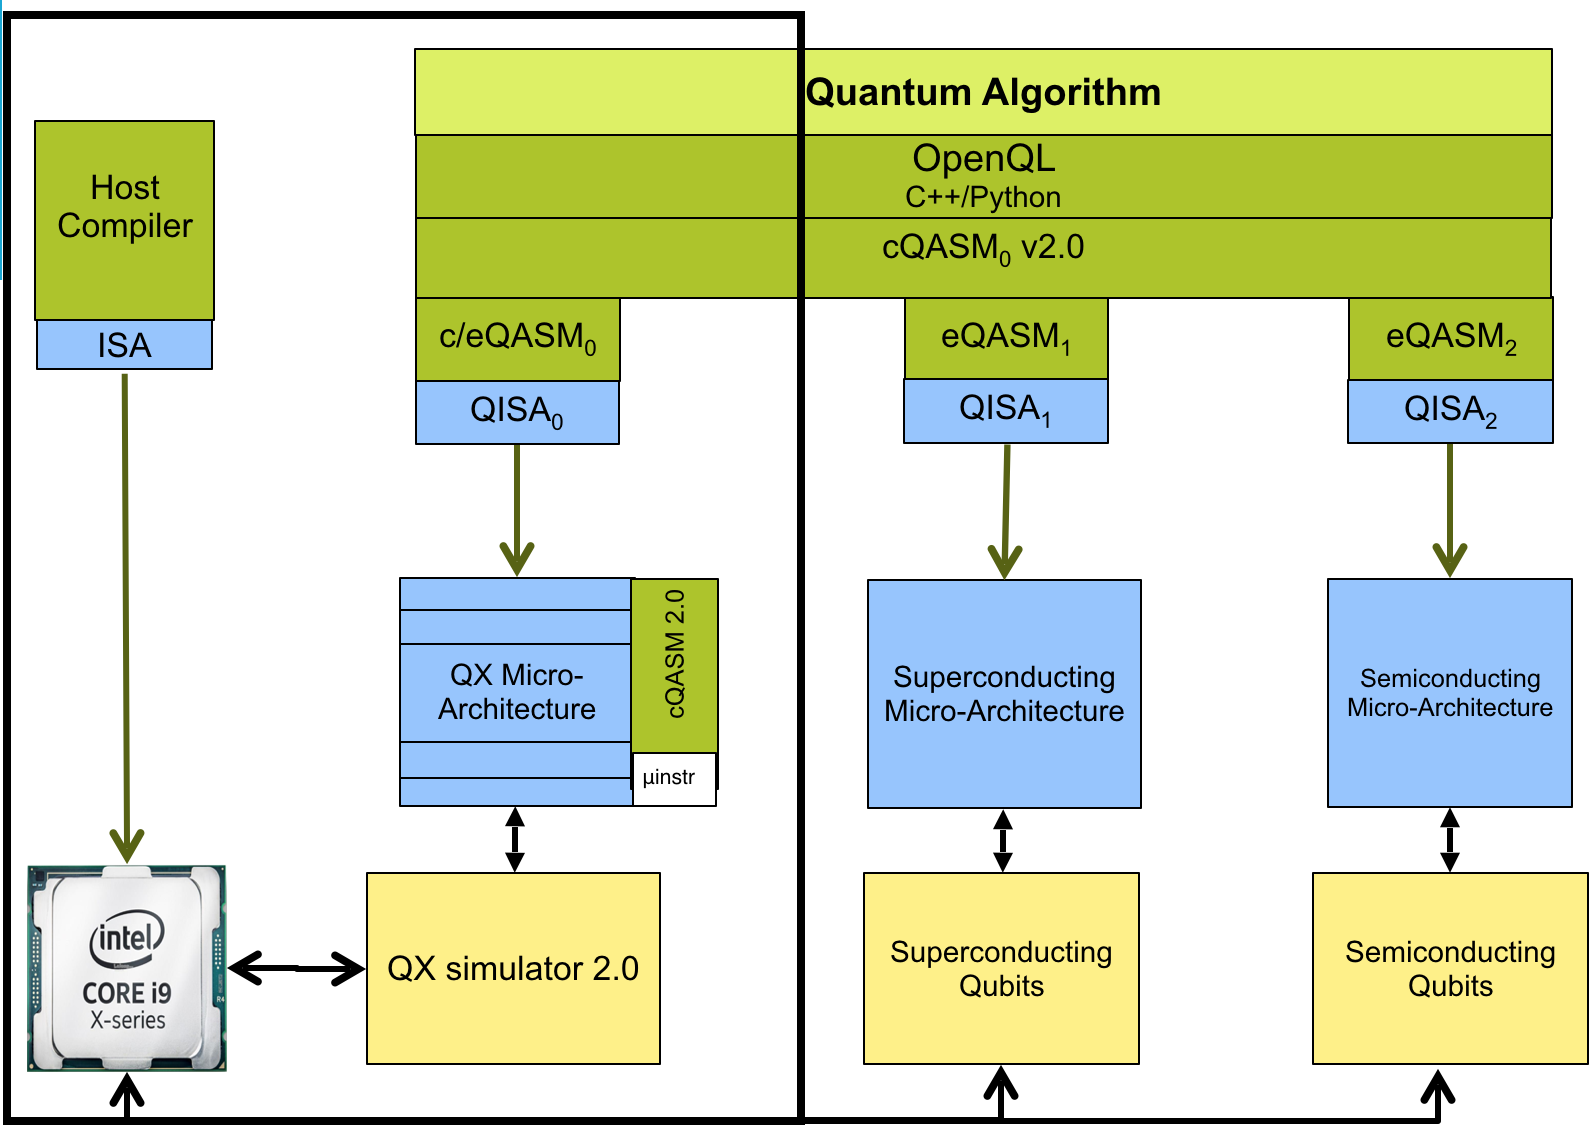
\includegraphics[width=\textwidth]{figures/layers.png}
\caption{\label{fig:org4501358}
Compilation layers}
\end{figure}


\begin{itemize}
\item cQASM
\label{sec:org4b78059}


\item OpenQL
\label{sec:orgf95ee3c}

\begin{figure}[htbp]
\centering
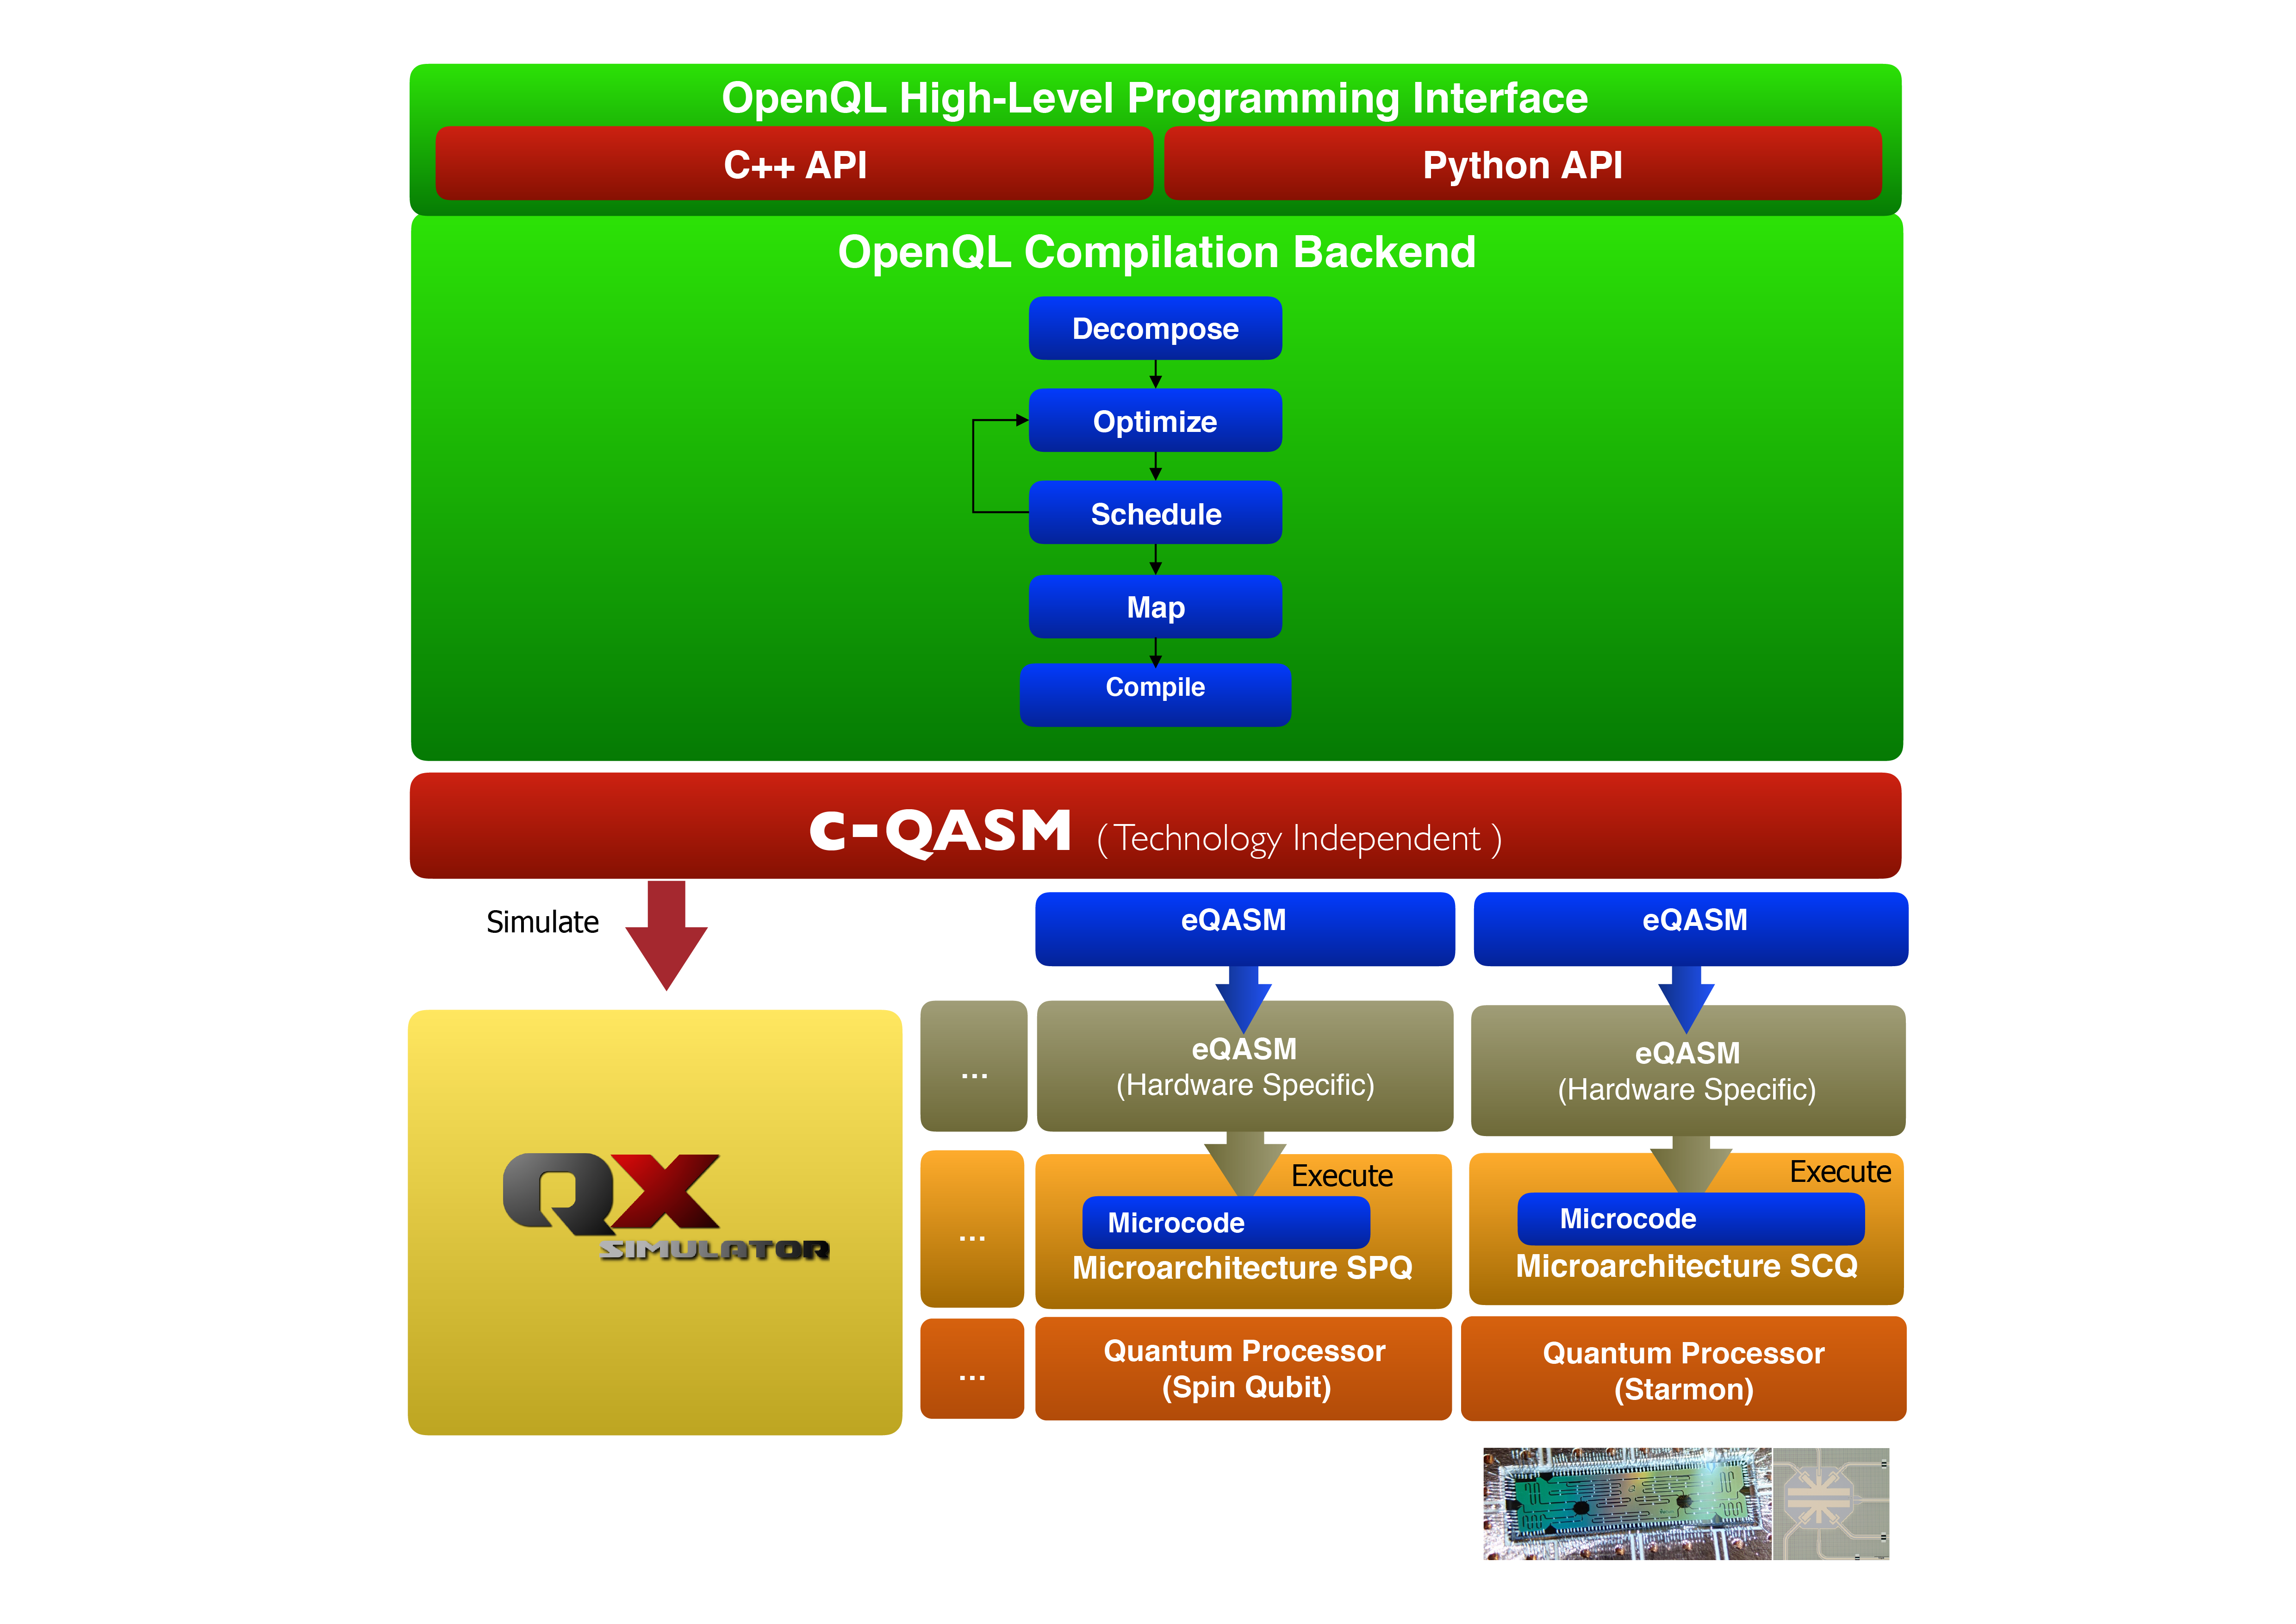
\includegraphics[width=0.9\textwidth]{figures/openql.png}
\caption{\label{fig:org1235bcb}
OpenQL diagram}
\end{figure}

\begin{figure}
\centering
\begin{minipage}{\textwidth}

\begin{minted}[frame=lines,fontsize=\scriptsize,linenos,breaklines,breakanywhere]{python}

from openql import openql as ql
import os
import argparse

def circuit(config_file, scheduler='ASAP', uniform_sched= 'no', mapper='base', initial_placement='no', output_dir_name='test_output', optimize='no', measurement=True, log_level='LOG_WARNING'):
    curdir = os.path.dirname(__file__)
    output_dir = os.path.join(curdir, output_dir_name)
    ql.set_option('output_dir', output_dir)
    ql.set_option('optimize', optimize)
    ql.set_option('scheduler', scheduler)
    ql.set_option('scheduler_uniform', uniform_sched)
    ql.set_option('mapper', mapper)
    ql.set_option('initialplace', initial_placement)
    ql.set_option('log_level', log_level)

    config_fn = os.path.join(curdir, config_file)

    platform  = ql.Platform('starmon', config_fn)
    sweep_points = [1,2]
    num_circuits = 1
    num_qubits = 6
    p = ql.Program('graycode6', platform, num_qubits)
    p.set_sweep_points(sweep_points, num_circuits)
    k = ql.Kernel('graycode6', platform, num_qubits)
    k.gate('cnot',[1,0])
    k.gate('cnot',[2,1])
    k.gate('cnot',[3,2])
    k.gate('cnot',[4,3])
    k.gate('cnot',[5,4])

    if measurement:
	for q in range(num_qubits):
	    k.gate('measure', [q])

    p.add_kernel(k)
    p.compile()

\end{minted}

\caption{OpenQL description in python code describing the Gray code algorithm.}
\label{code:openql_gray_code}
\end{minipage}
\end{figure}
\end{itemize}

\subsection*{quantumsim}
\label{sec:org6ff3881}

Quantumsim \cite{O_Brien_2017} is a simulator of superconducting systems designed to study the SC-7 and SC-17 chips and based on their behaviour on experiments.
It performs calculations on \textbf{density matrices} instead of the compact representation of the quantum states because they permit the use of mixed states -- able to represent any kind of errors.
As it can be inherited in the \href{quantum_computing.org}{Qubits} subsection, the density matrix size grows exponentially with the number of qubits it represents -- \(2^n \times 2^n\) where \(n\) is the number of qubits.
Once the qubits state is ready as a density matrix, quantumsim applies the quantum gates in the \textbf{Pauli transfer matrix representation}.
The Pauli representation builds positive matrices that preserves the trace properties of the original matrix -- Completely Positive Trace-Preserving (CPTP) transformation -- \cite{Merkel_2013} to represent the gates.
In order to avoid non-efficient calculations, in place of building a huge density matrix considering all the qubits from the very beginning, quantumsim will enlarge dynamically the density matrix whenever a gate requires a new qubit.
As this calculations are computationally hard, quantumsim has the possibility of boosting calculations with a Graphics Processing Unit (GPU).


\begin{equation}
\label{eq:orgb6f006b}
(R_{\Lambda})_{ij} = \frac{1}{2} Tr(\sigma_i \Lambda \sigma_j)
\end{equation}

where \(\Lambda\) is the CPTP transformation and \(\sigma_i\) are the Pauli operators, viz. \(\sigma_0 = I\), \(\sigma_1 = X\), \(\sigma_2 = Y\), \(\sigma_3 = Z\), equivalent to rotations around the main axes of the Bloch sphere.




\begin{itemize}
\item Error model
\label{sec:org8d7cded}

Quantumsim considers six main error sources in the SC-7 and SC-17, of which three comes from the different operations -- single/two-qubit gates and measurement -- and the others are either decoherence or apparatus related errors -- photon decay and the flux noise.
Each operation has its own model, based on the learning extracted from several experiments.
The same happens to the other studied phenomena that are incorporated in different ways in the gate matrices.
In this section we will describe the error sources and how they are simulated in quantumsim.
From decoherence to the apparatus related errors -- that affect the gates error.
Also, Tab. \ref{tab:org23a69ab} pinpoints exactly the value of the parameters used in the error model.


\begin{itemize}
\item Qubit Idling
\label{sec:org1fe3b4e}

While idling for a time \(t\), a transmon in \(|1\rangle\) or in superposition could relax to \(|0\rangle\) or acquire random quantum phase shifts due to \(1/f\) noise sources (flux noise) or others.
The dephasing effect only appears in a superposition state.
\begin{equation}
\label{eq:org34ae206}

R_{\Lambda_{T_1}} = \begin{bmatrix}
 1 & 0 & 0 & 0 \\
 0 & \sqrt{1 - p_1} & 0 & 0 \\
 0 & 0 & \sqrt{1 - p_1} & 0 \\
 p_1 & 0 & 0 & 1 - p_1 \\
\end{bmatrix}

\end{equation}

\begin{equation}
\label{eq:orgde00172}

R_{\Lambda_{T_{\phi}}} = \begin{bmatrix}
 1 & 0 & 0 & 0 \\
 0 & \sqrt{1 - p_{\phi}} & 0 & 0 \\
 0 & 0 & \sqrt{1 - p_{\phi}} & 0 \\
 0 & 0 & 0 & 1 \\
\end{bmatrix}

\end{equation}

with \(p_1 = 1 - e^{-\frac{t}{T_1}}\) and \(p_{\phi} = 1 - e^{-\frac{t}{T_{\phi}}}\) that are the probabilities for relaxation and pure dephasing, respectively.
Idling for a duration \(t\):

\begin{equation}
\label{eq:orga135486}

R_{AP (t)} = R_{\Lambda_{T_1}} R_{\Lambda_{T_{\phi}}}

\end{equation}

\item Photon decay
\label{sec:org1346030}
While measuring a qubit state under the presence of photons in a readout resonator, the coupled qubit is affected suffering a \(p_{\phi, photon}\) dephasing.
This dephasing is present whenever the coupled qubit is brought into superposition before the readout resonator has returned to the vacuum state following the last measurement.
This dephasing is then implemented via the same Pauli transfer matrix as \(R_{\Lambda_{T_{\phi}}}\) in eq. \ref{eq:orga135486}.

\item Flux Noise
\label{sec:orgf343682}

Whenever a two-qubit operation is done, qubits are moved in frequency away to their sweet spot (\(f_{q,max}\)) with flux pulses as it was seen in the \href{chapter-3.org}{Constraints of the Surface-7 and -17 chips} section.
And the only affected qubits are not the targeted ones, but also the NN that need to avoid the effects of the operation.
While outside their sweet spot, the qubits are highly affected by the noise inserted by the flux pulses.
This noise causes a random phase shift in the qubit state.
As soon as the power spectrum of the flux noise is \(1/f\) -- main contribution is related with low-frequencies --, adjusting the qubit frequency to a lower frequency makes the qubit even more sensitive to it.

\item Single-qubit \(R_y(\pi /2)\) rotations
\label{sec:org50f94e2}

Quantumsim models single-qubit gates adding idle matrices of duration \(\frac{\tau_{g,1Q}}{2}\) before and after the CPTP gate representation, allowing the insertion of amplitude and phase damping (\(T_1\) and \(T_{\phi}\))).
The addition of this error is equivalent to shrinking a quantum state towards the origin.
Quantumsim considers this shrinking with a factor of \(1 - p_{axis}\) along the y-axis and \(1 - p_{plane}\) along the x- and z-axes as it is described in eq. \ref{eq:orge97a618}.

\begin{equation}
\label{eq:orge97a618}

R_{R_y (\pi /2)} = R_{AP (\frac{\tau_{g,1Q}}{2})} R_{R_y (\pi /2)}' R_{dep} R_{AP (\frac{\tau_{g,1Q}}{2})}

\end{equation}

where

$$R_{dep} = \begin{bmatrix}
 1 & 0 & 0 & 0 \\
 0 & 1 - p_{plane} & 0 & 0 \\
 0 & 0 & 1 - p_{axis} & 0 \\
 0 & 0 & 0 & 1 - p_{plane} \\
\end{bmatrix}$$

and \(R_{R_y (\pi/2)}'\) is the Pauli transfer matrix describing the theoretical \(\pi /2\) rotation along the y axis.

\item CZ gates
\label{sec:orgf460e35}

As it was described in the \href{chapter-3.org}{Constraints of the Surface-7 and -17 chips} section, a CZ gate is executed flu pulsing the frequency of the qubits in to a frequency in the middle of their sweet spots.
That make both qubit states interact with each other in a CZ gate fashion, holding the qubits for a \(\tau_{g,2Q}\) period of time.
Quantumsim's model of the CZ gate consists of a CZ representation adding the single-qubit phase error \(\delta_{\phi_{1Q}}\) as well as the two-qubit phase error \(\delta_{\phi_{2Q}} = \frac{\delta_{\phi_{1Q}}}{2}\).
It will be also surrounded by idling intervals of duration \(\frac{\tau_{g,2Q}}{2}\).
Quantumsim neglects leakage during the two-qubit gates because previous experiments have reduced leakage probability per CZ to \(\approx\) 0.3\%.

\item Measurement
\label{sec:org1e662f8}

The behaviour of the measurements in the simulations follow the Born rule \cite{O_Brien_2017}, giving projection probabilities calculated based on the quantum state probabilities.
The measurements are implemented as black-boxes surrounded by idling steps (as the other quantum gates).
The black-box consists of a dephasing -- due to the photon decay phenomena -- followed by a period of decay and excitation with probability \(p_{\uparrow / \downarrow}^{(1)}\).
After that, the qubit state is collapsed with an error probability \(\epsilon_{RO}\) and, then, the qubit state is subject to further decay or excitation with probabilities \(p_{\uparrow / \downarrow}^{(2)}\).
Finally, after measuring, quantumsim removes that qubit out of the main density matrix.
Quantumsim ignore effects leading to measurement-induced mixing and non-linearity of the readout resonator, as well as residual photon numbers.

\begin{figure}[htbp]
\centering
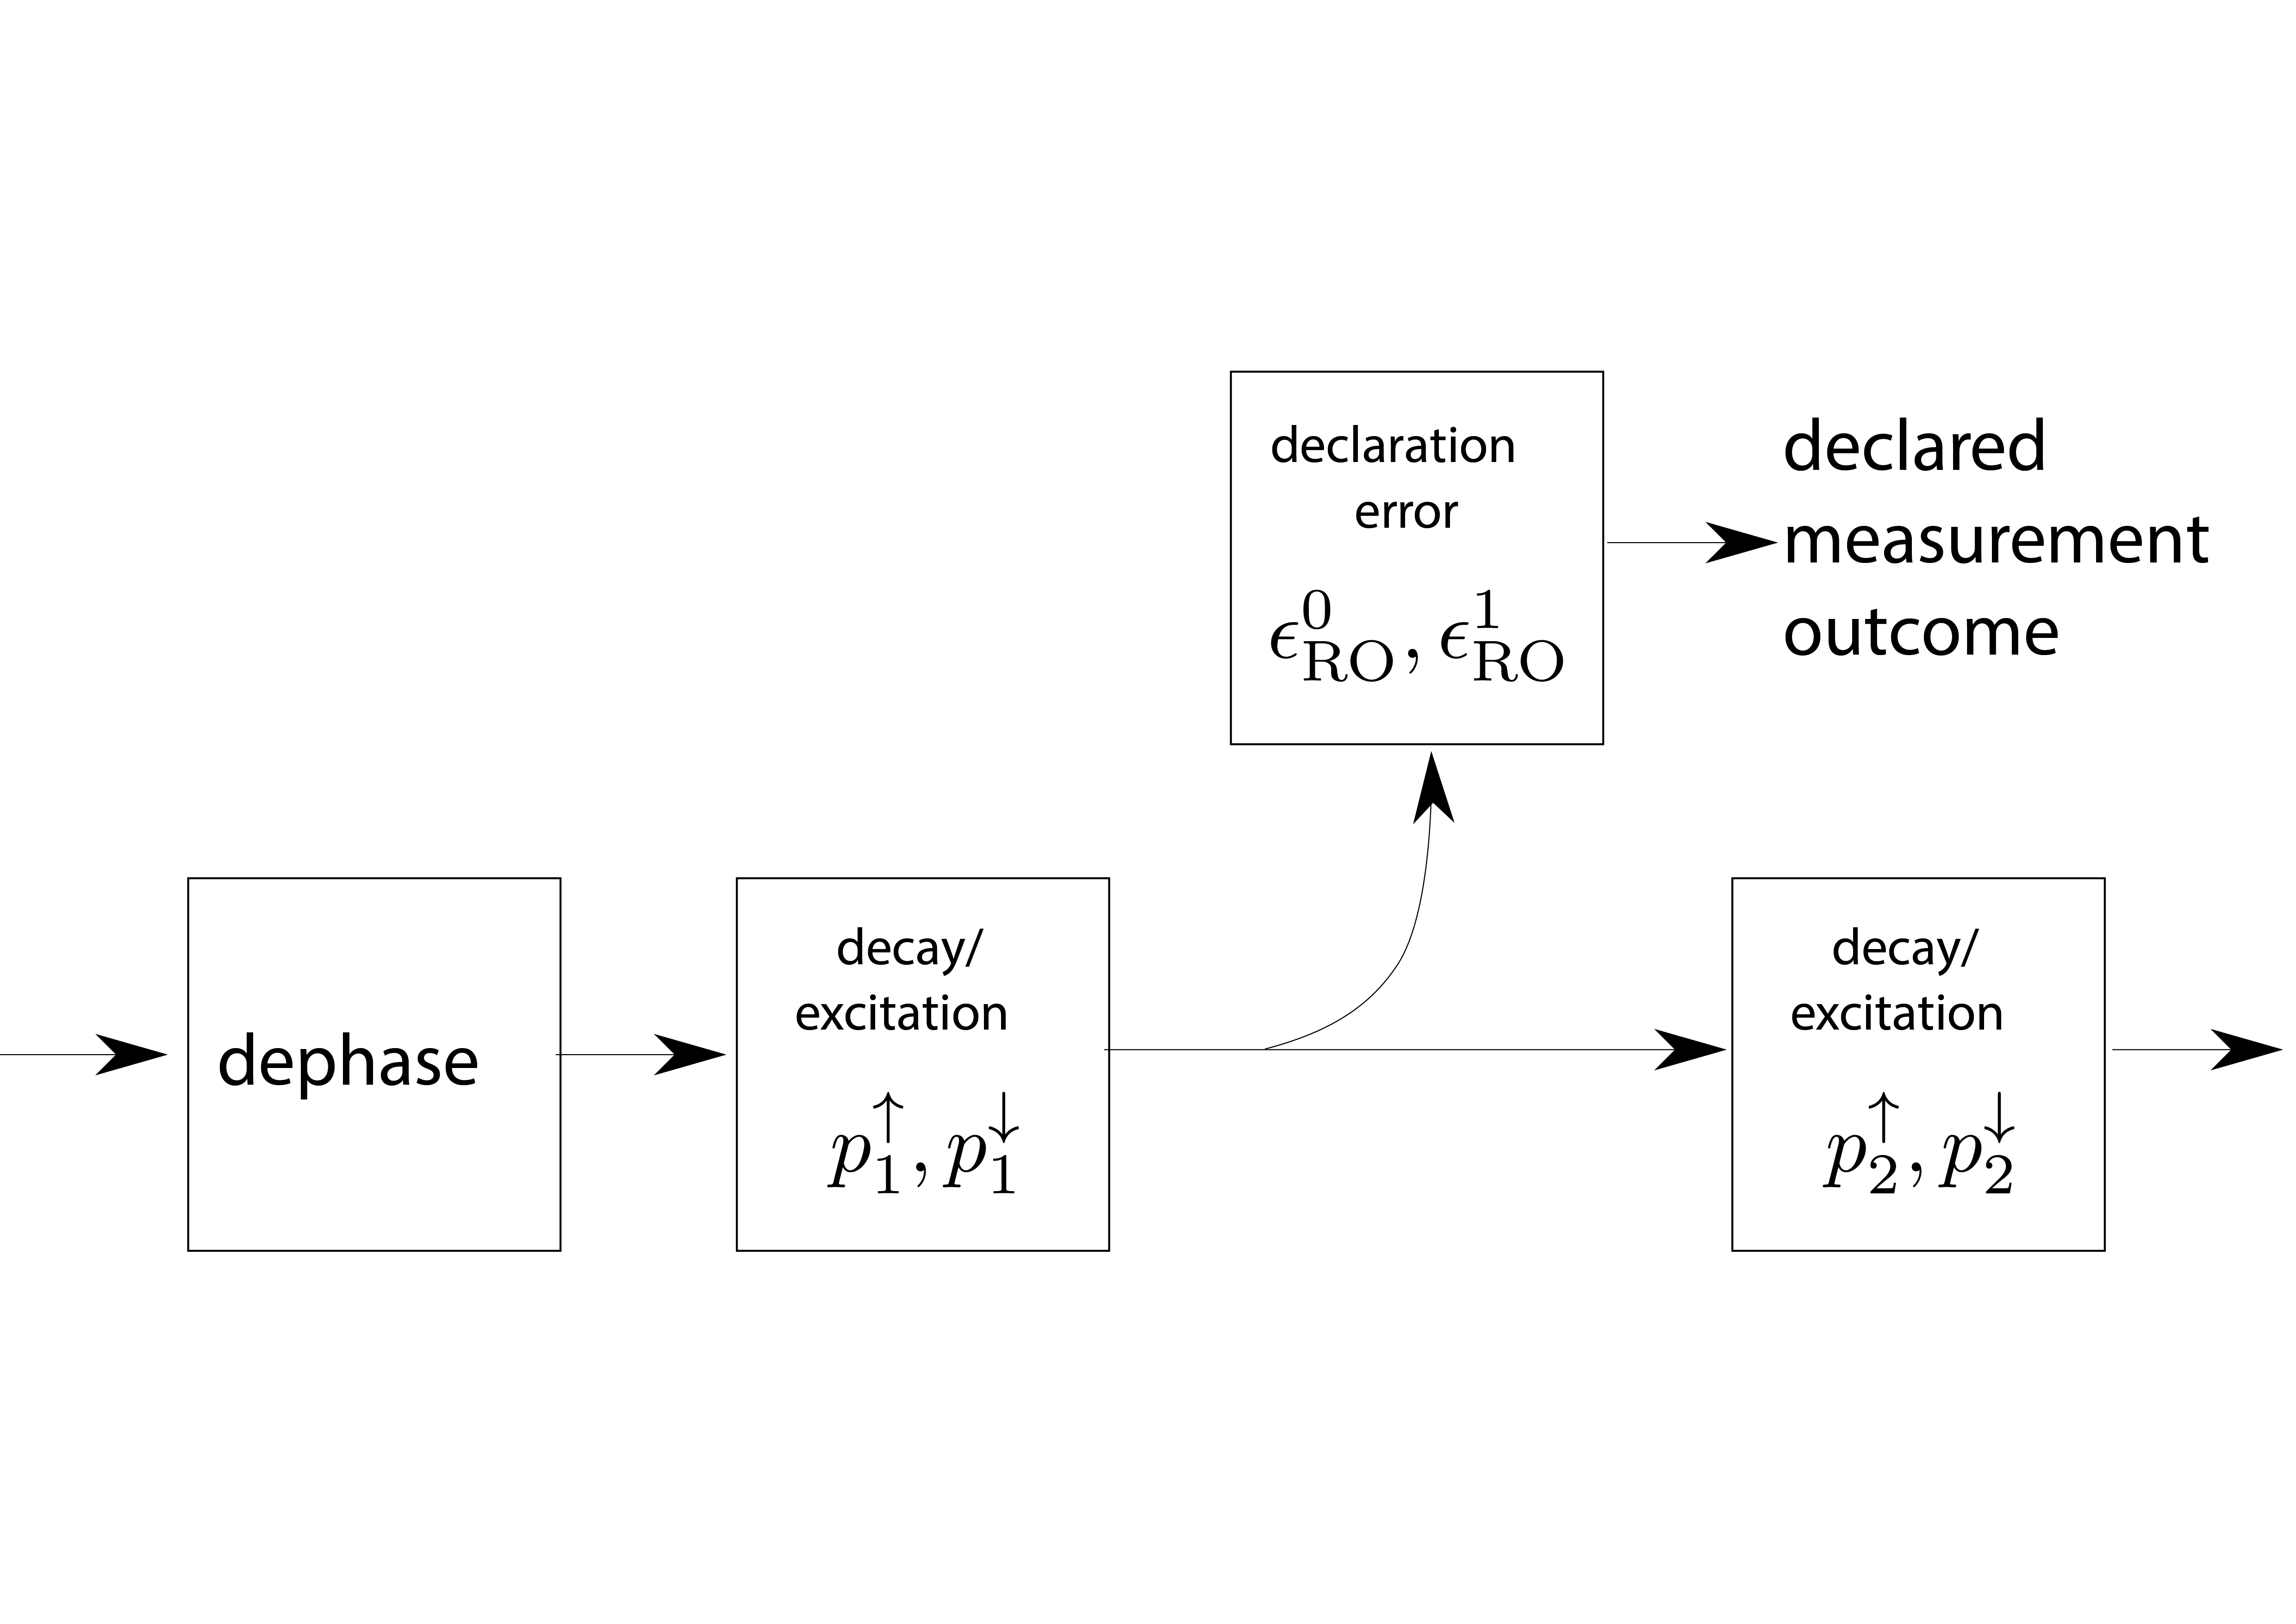
\includegraphics[width=0.5\textwidth]{figures/measure_model.png}
\caption{\label{fig:orge4ffd14}
Black box model from \cite{O_Brien_2017}}
\end{figure}



\begin{table}[htbp]
\caption{\label{tab:org23a69ab}
Main error model parameters for simulation \cite{O_Brien_2017}}
\centering
\tiny
\begin{tabular}{lccp{7cm}}
\hline
Parameter & Symbol & Value & Explanation and notes\\
\hline
Qubit relaxation time & \(T_1\) & 30 \(\mu s\) & Only affects qubits in the excited state. Consistent set of values: [20 - 100 \(\mu s\)]\\
Qubit dephasing time (white noise) & \(T_{\phi}\) & 60 \(\mu s\) & Consistent set of values would be \(2 T_1\) or \(\infty\) (all white noise dephasing eliminated)\\
Decay time & \(T_2\) & 30 \(\mu s\) & \(\frac{1}{T_2} = \frac{1}{T_{\phi}} + \frac{1}{2 T_1}\)\\
Single-qubit gate time & \(T_{g,1Q}\) & 20 ns & \\
Two-qubit gate time & \(T_{g,2Q}\) & 40 ns & \\
Measurement time & \(\tau_m\) & 300 ns & \\
Depletion time & \(\tau_d\) & 300 ns & ?\\
Fast Measurement time & \(\tau_m^{\text{fast}}\) & 100 ns & \\
Fast Depletion time & \(\tau_d^{\text{fast}}\) & 100 ns & ?\\
Readout infidelity & \(\epsilon_{RO}\) & 5\,(-3) & \\
Physical qubit Fidelity & \(\mathcal{F}_{phys} (t)\) & - & \(\mathcal{F}_{phys} (t) = \frac{1}{6}\left(1 + e^{-\frac{t}{T_1}}\right) + \frac{1}{3}\left(1 + e^{-t\left(\frac{1}{2 T_1} + \frac{1}{T_{\phi}}\right)} \right)\)\\
Physical qubit error rate & \(\epsilon_{phys}\) & - & \(\epsilon_{phys} = - \tau_{circuit} \frac{d \mathcal{F}_{phys} (t)}{dt} \textbar_{t=0}=\frac{\tau_{circuit}}{3 T_1}+\frac{\tau_{circuit}}{3 T_{\phi}}\)\\
In-axis rotation error & \(p_{axis}\) & 1\,(-4) & Decay corresponding to shrinking along the y axis because of the single-qubit gates depolarizing noise\\
In-plane rotation error & \(p_{plane}\) & 5\,(-4) & Decay corresponding to shrinking along the x and z axis because of the single-qubit gates depolarizing noise\\
\hline
\end{tabular}
\end{table}
\end{itemize}


\item Github repository
\label{sec:orgebe7718}

Quantumsim can be found as \textbf{python library} in its \href{https://github.com/quantumsim/quantumsim}{github repository} with instructions to install it and an overview of how to use it.
\end{itemize}

\subsection*{Error Framework}
\label{sec:org2d710a0}
\begin{figure}[htbp]
\centering
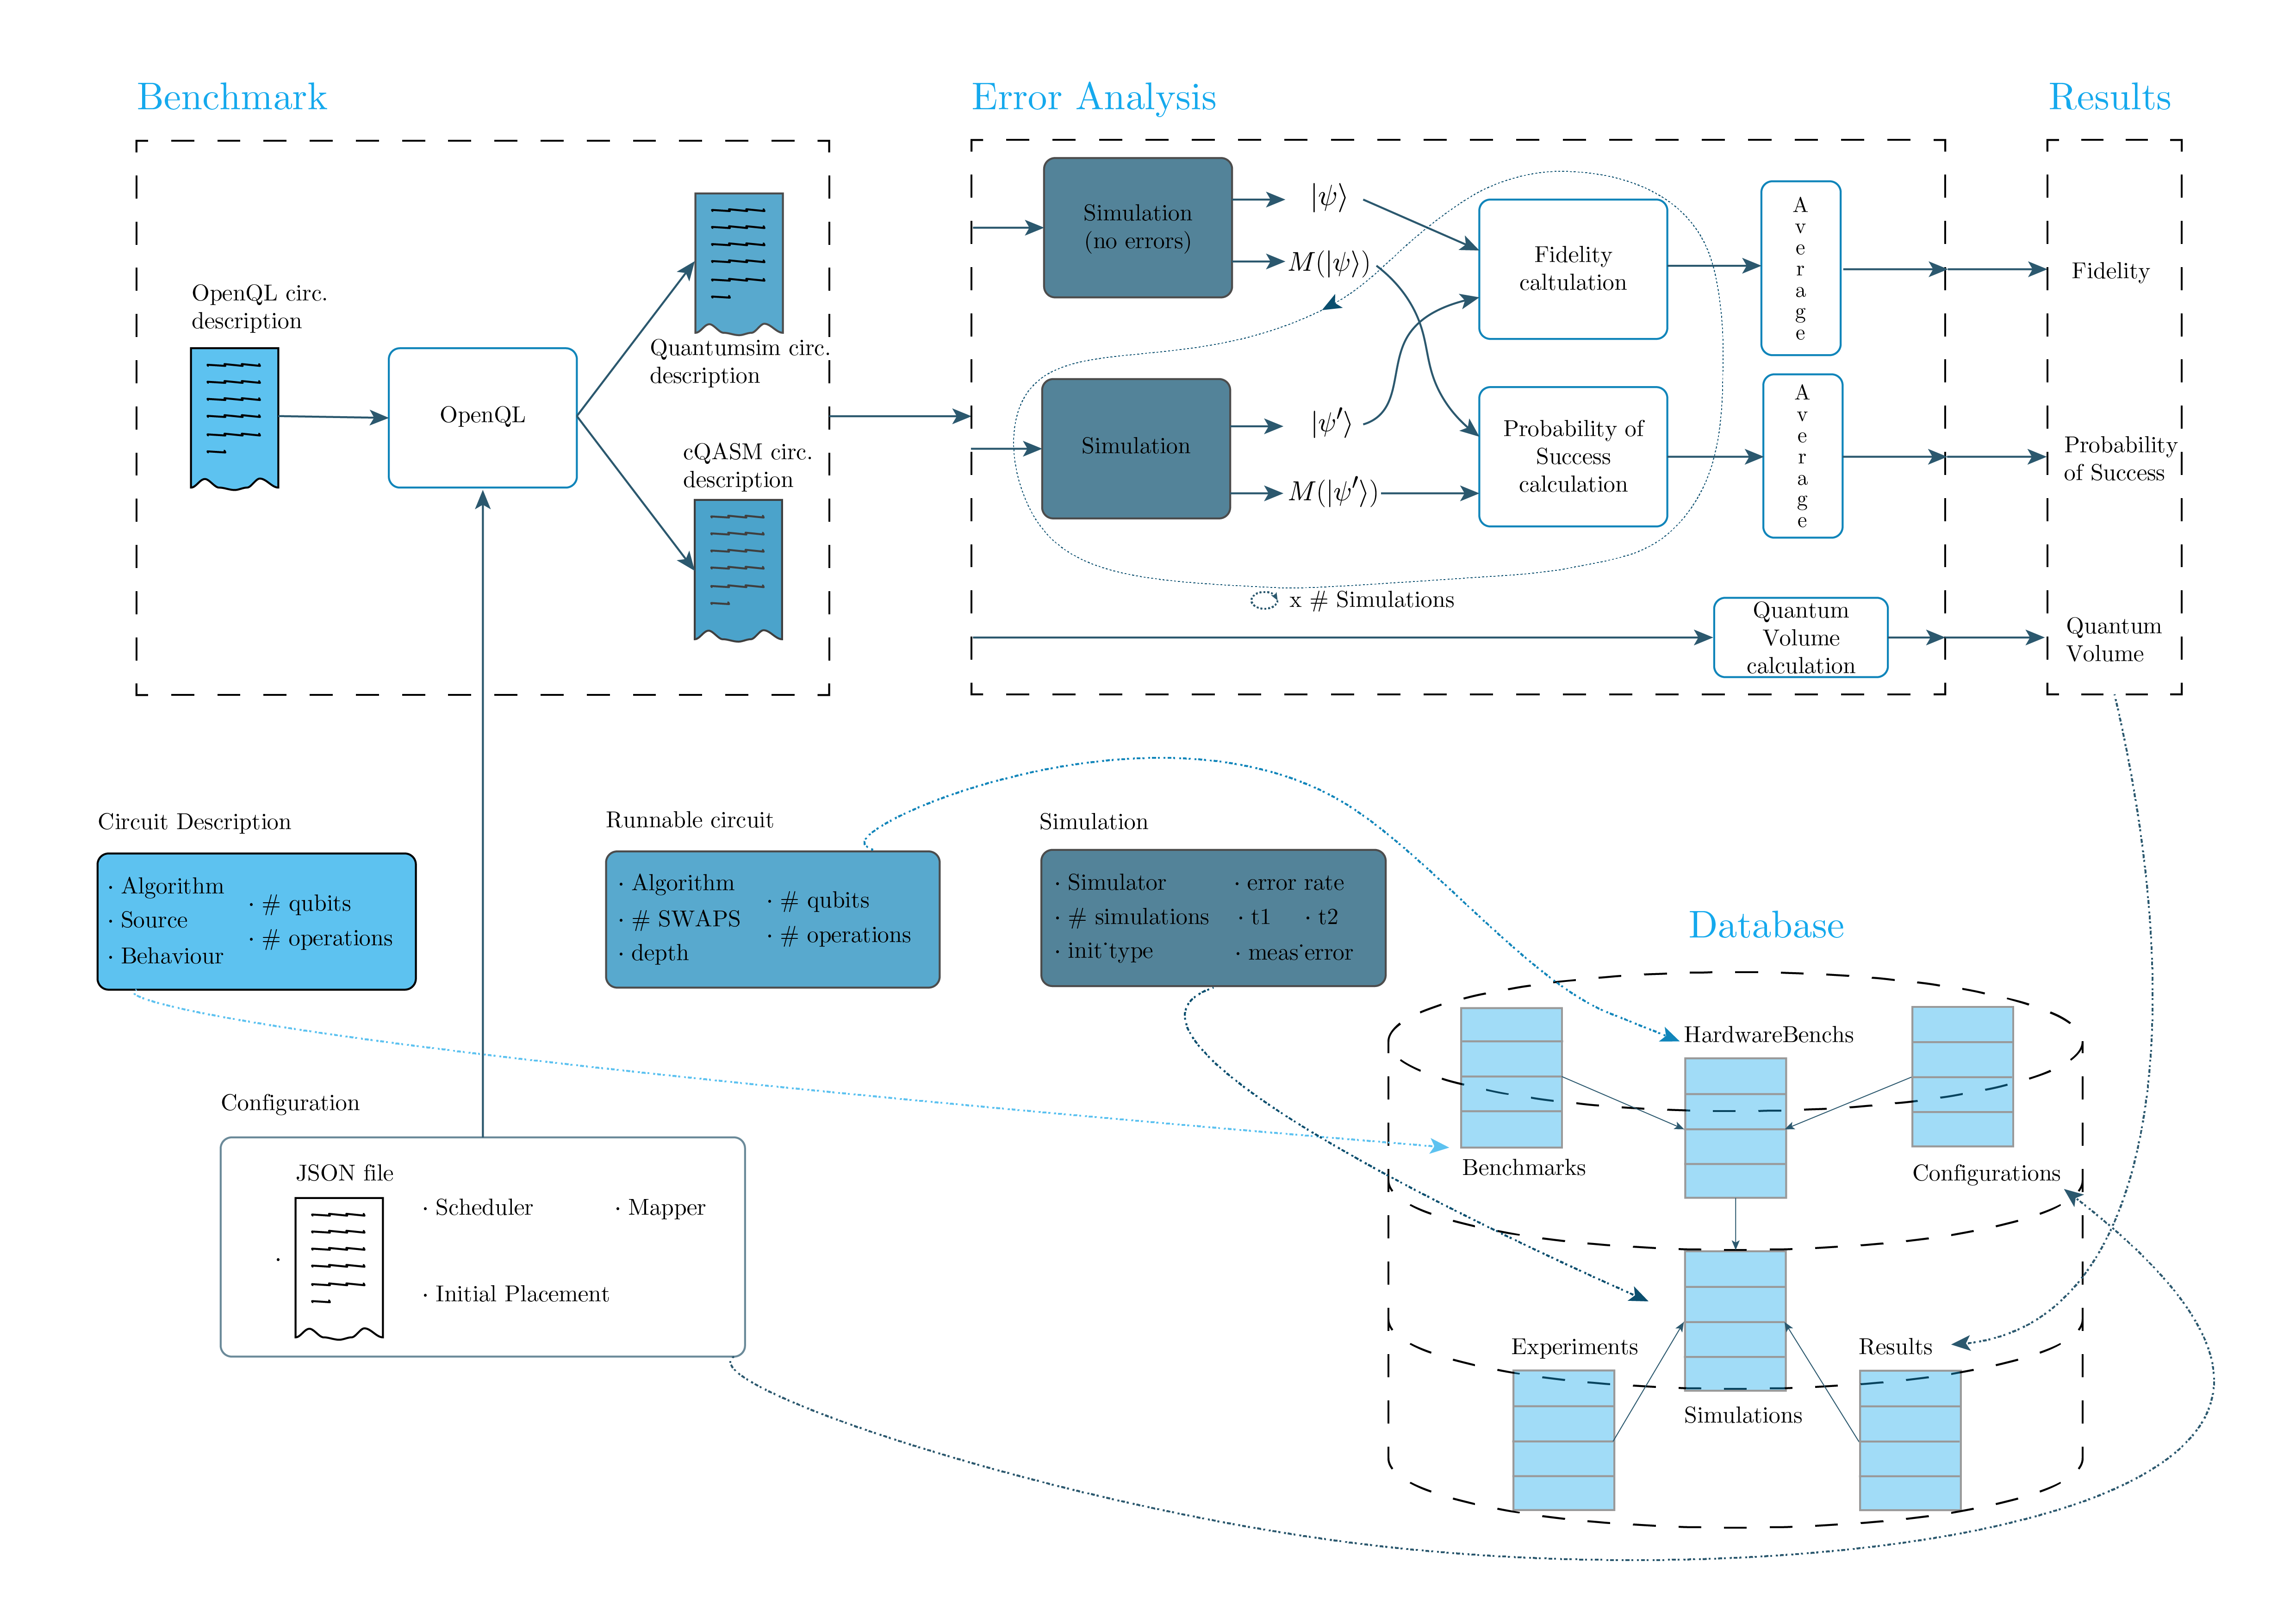
\includegraphics[width=\textwidth]{figures/error_framework_diagram.png}
\caption{\label{fig:orgf39a87d}
Error Framework}
\end{figure}

\begin{itemize}
\item Benchmark Object
\label{sec:org81ee96d}

\begin{figure}[htbp]
\centering
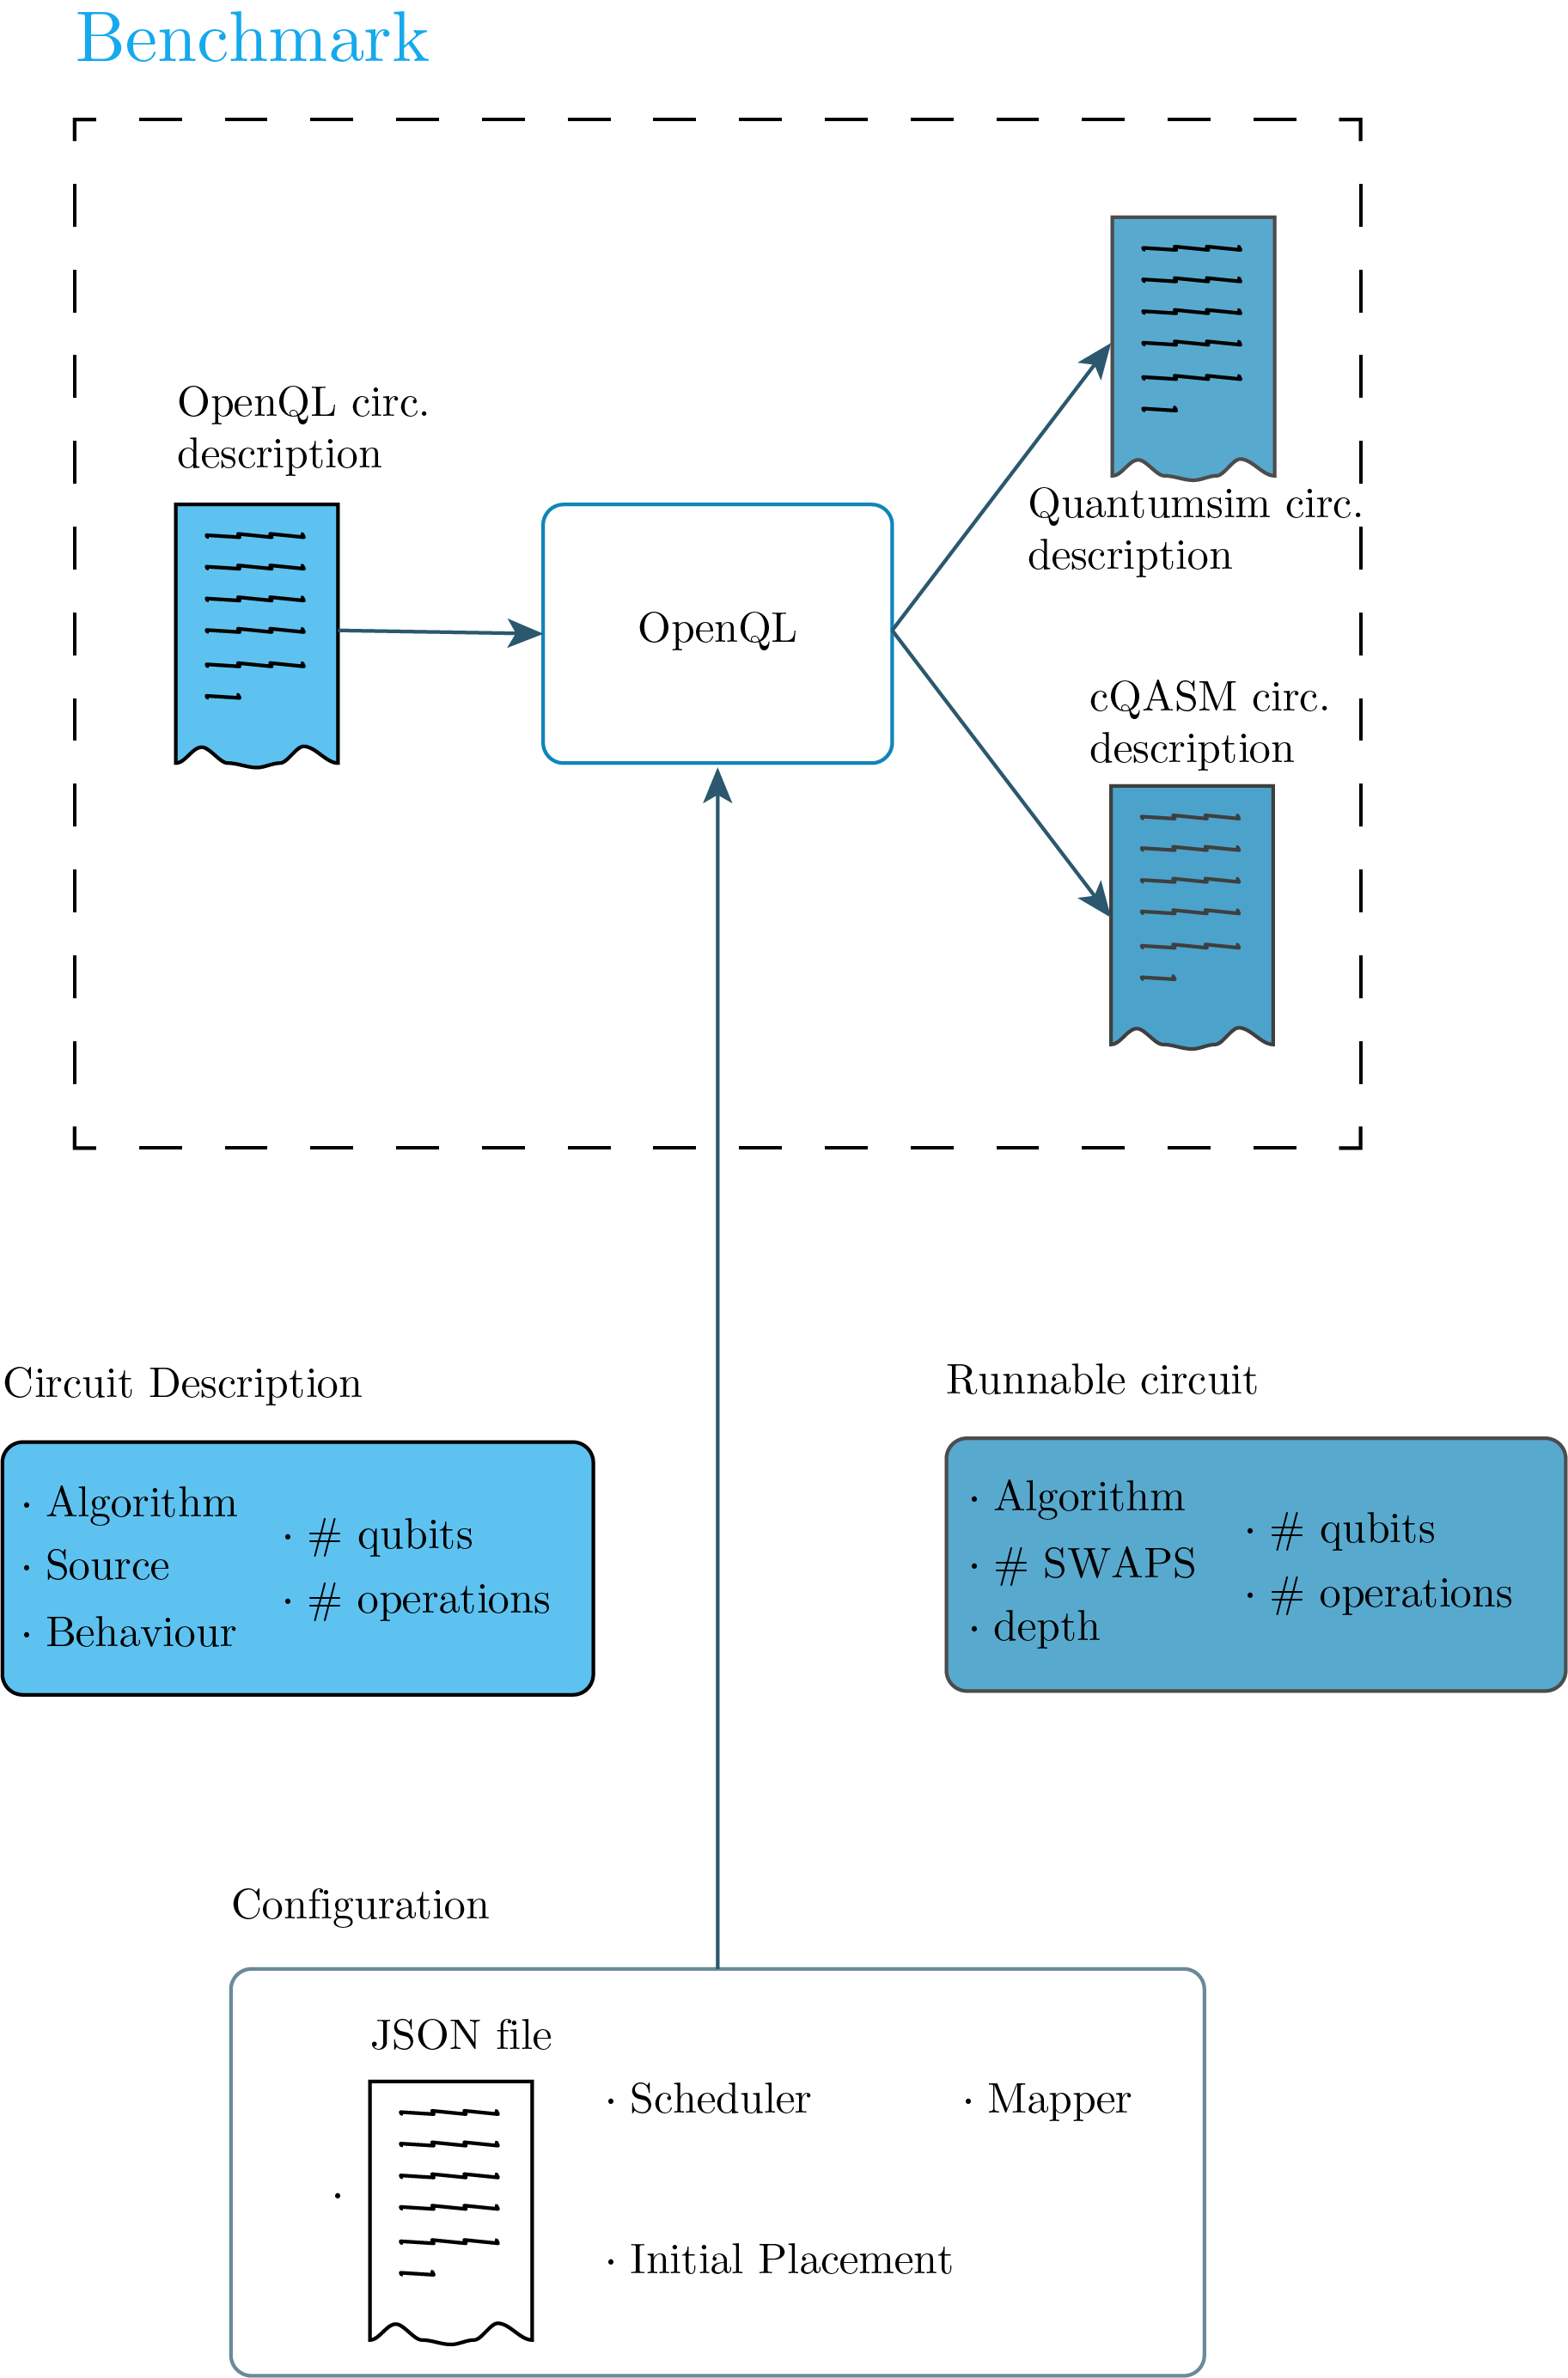
\includegraphics[width=.5\textwidth]{figures/benchmark_object.png}
\caption{\label{fig:org18bc473}
Benchmark Object \ldots{}}
\end{figure}

\item Mapping Analysis Object
\label{sec:org0a9c586}

\begin{figure}[htbp]
\centering
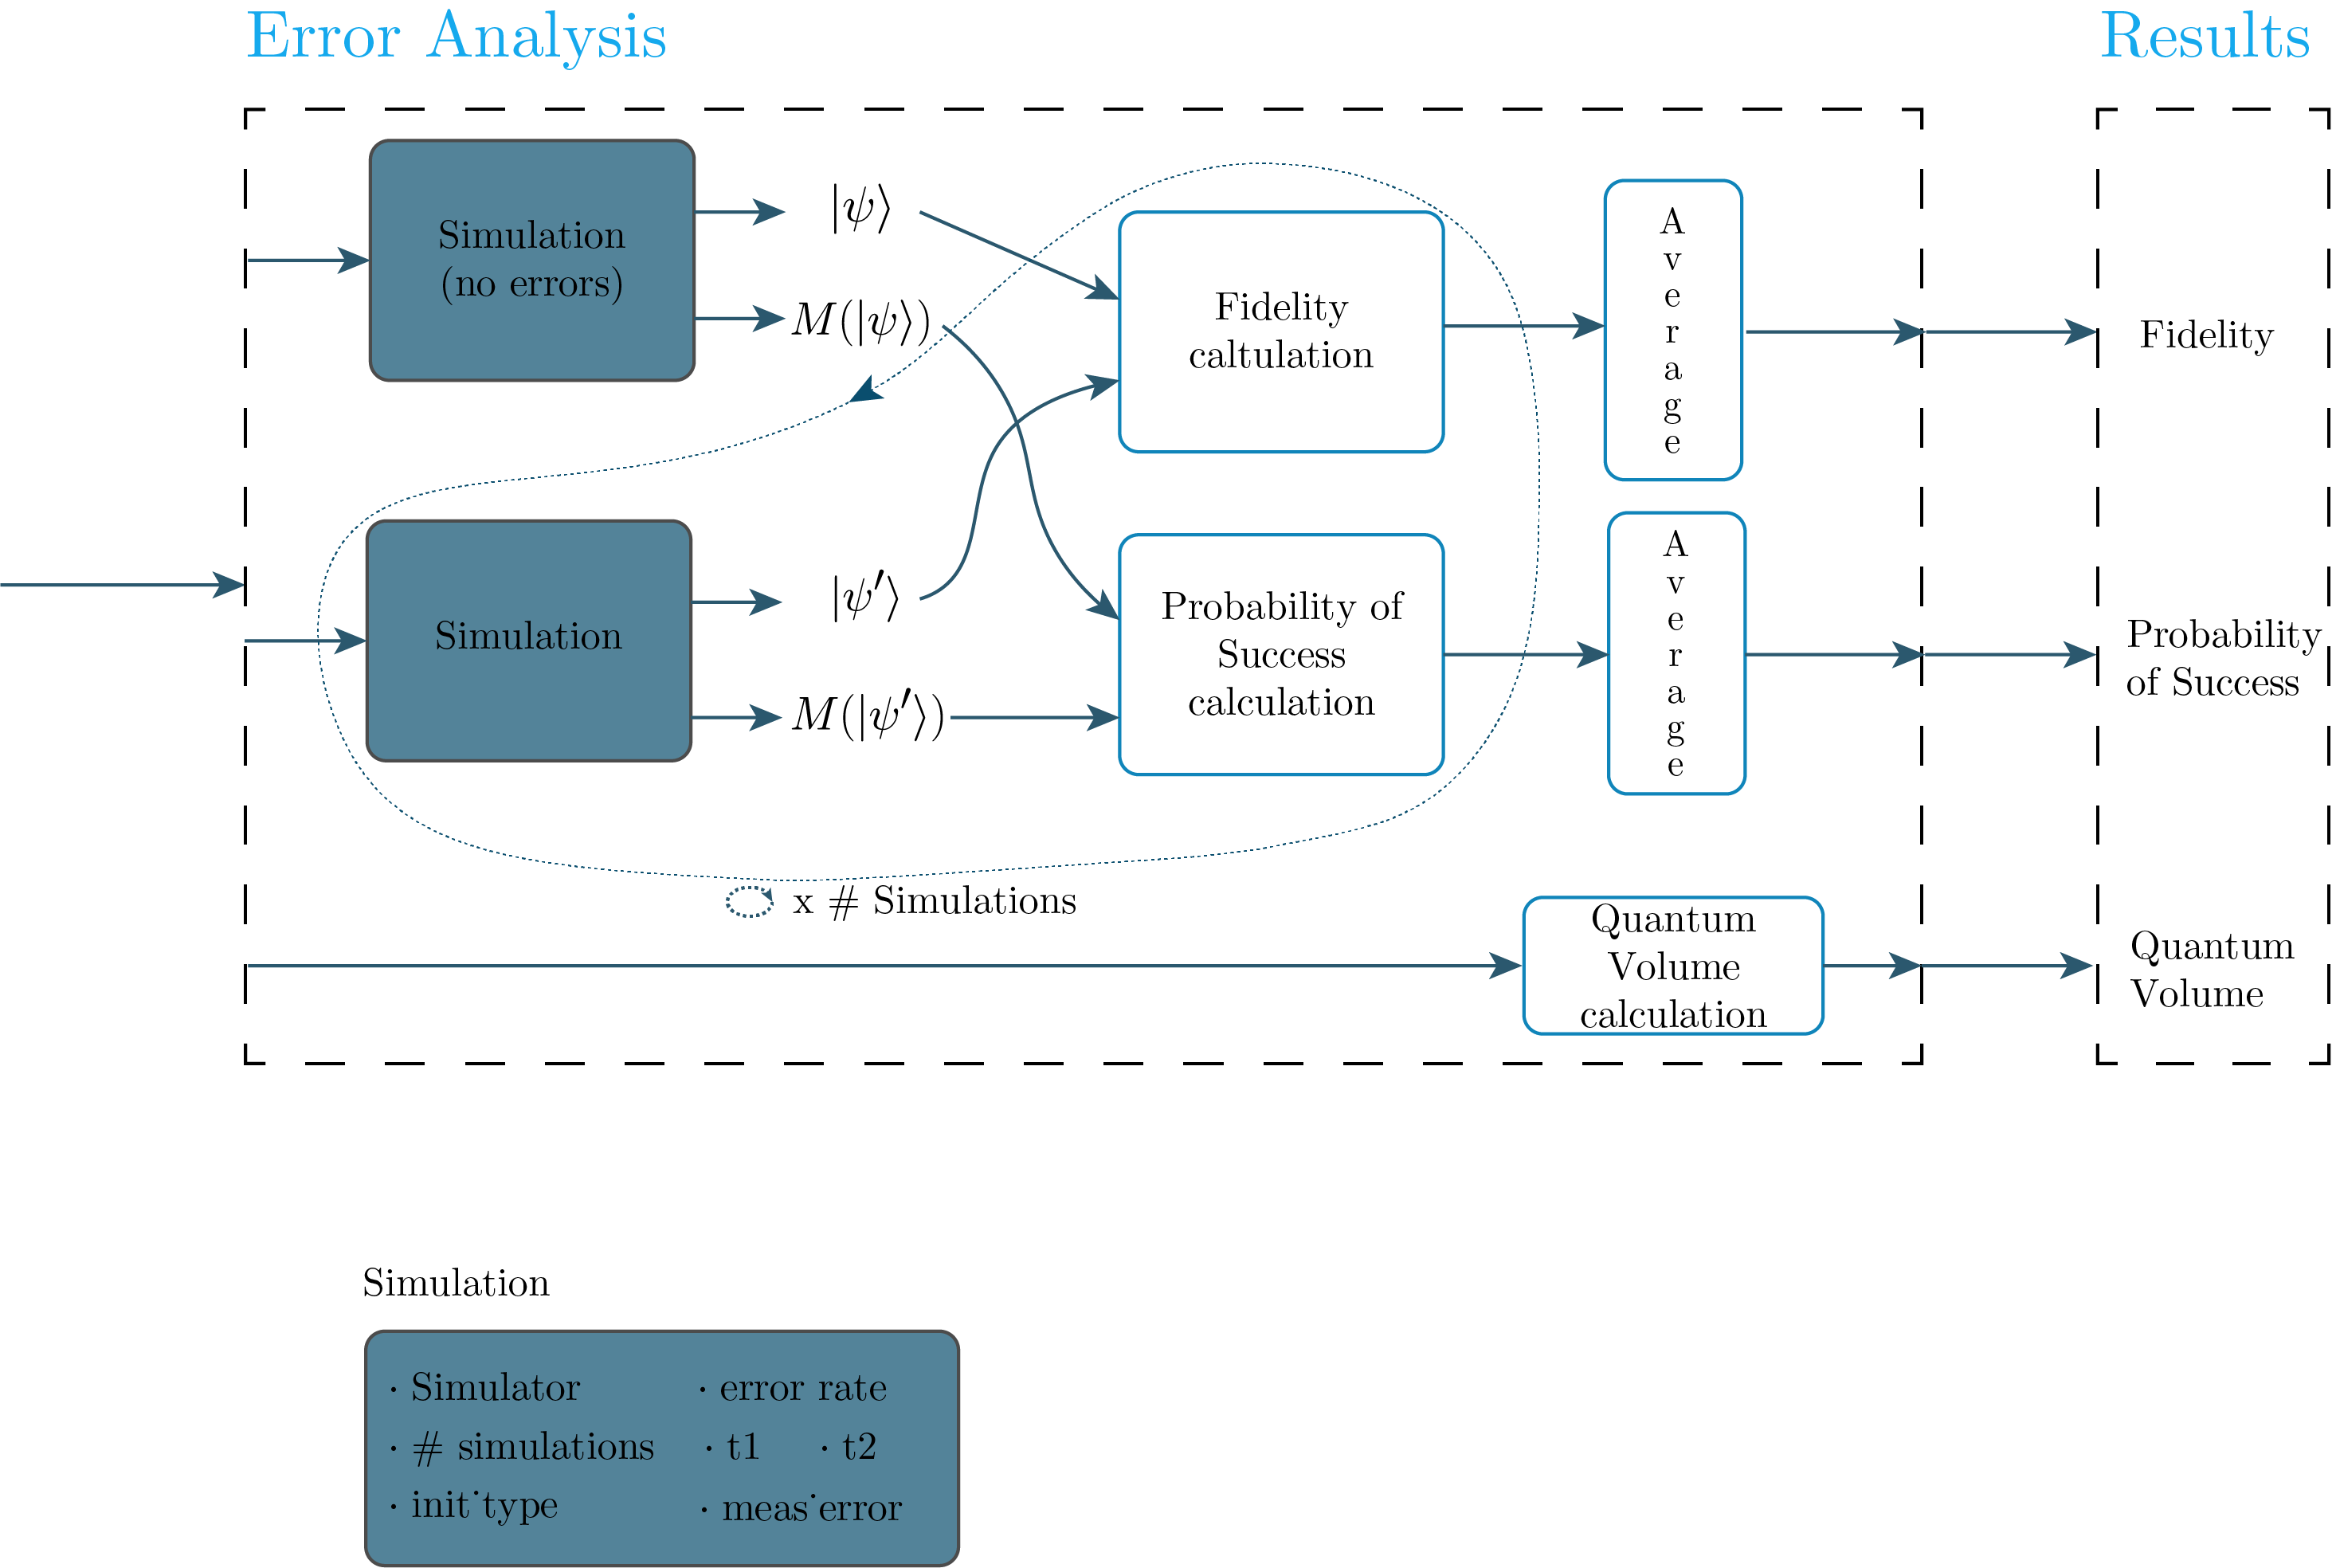
\includegraphics[width=.75\textwidth]{figures/error_analysis.png}
\caption{\label{fig:orga6f4096}
Mapping Analysis Object \ldots{}}
\end{figure}

\item Database
\label{sec:orgae24f73}

\begin{figure}[htbp]
\centering
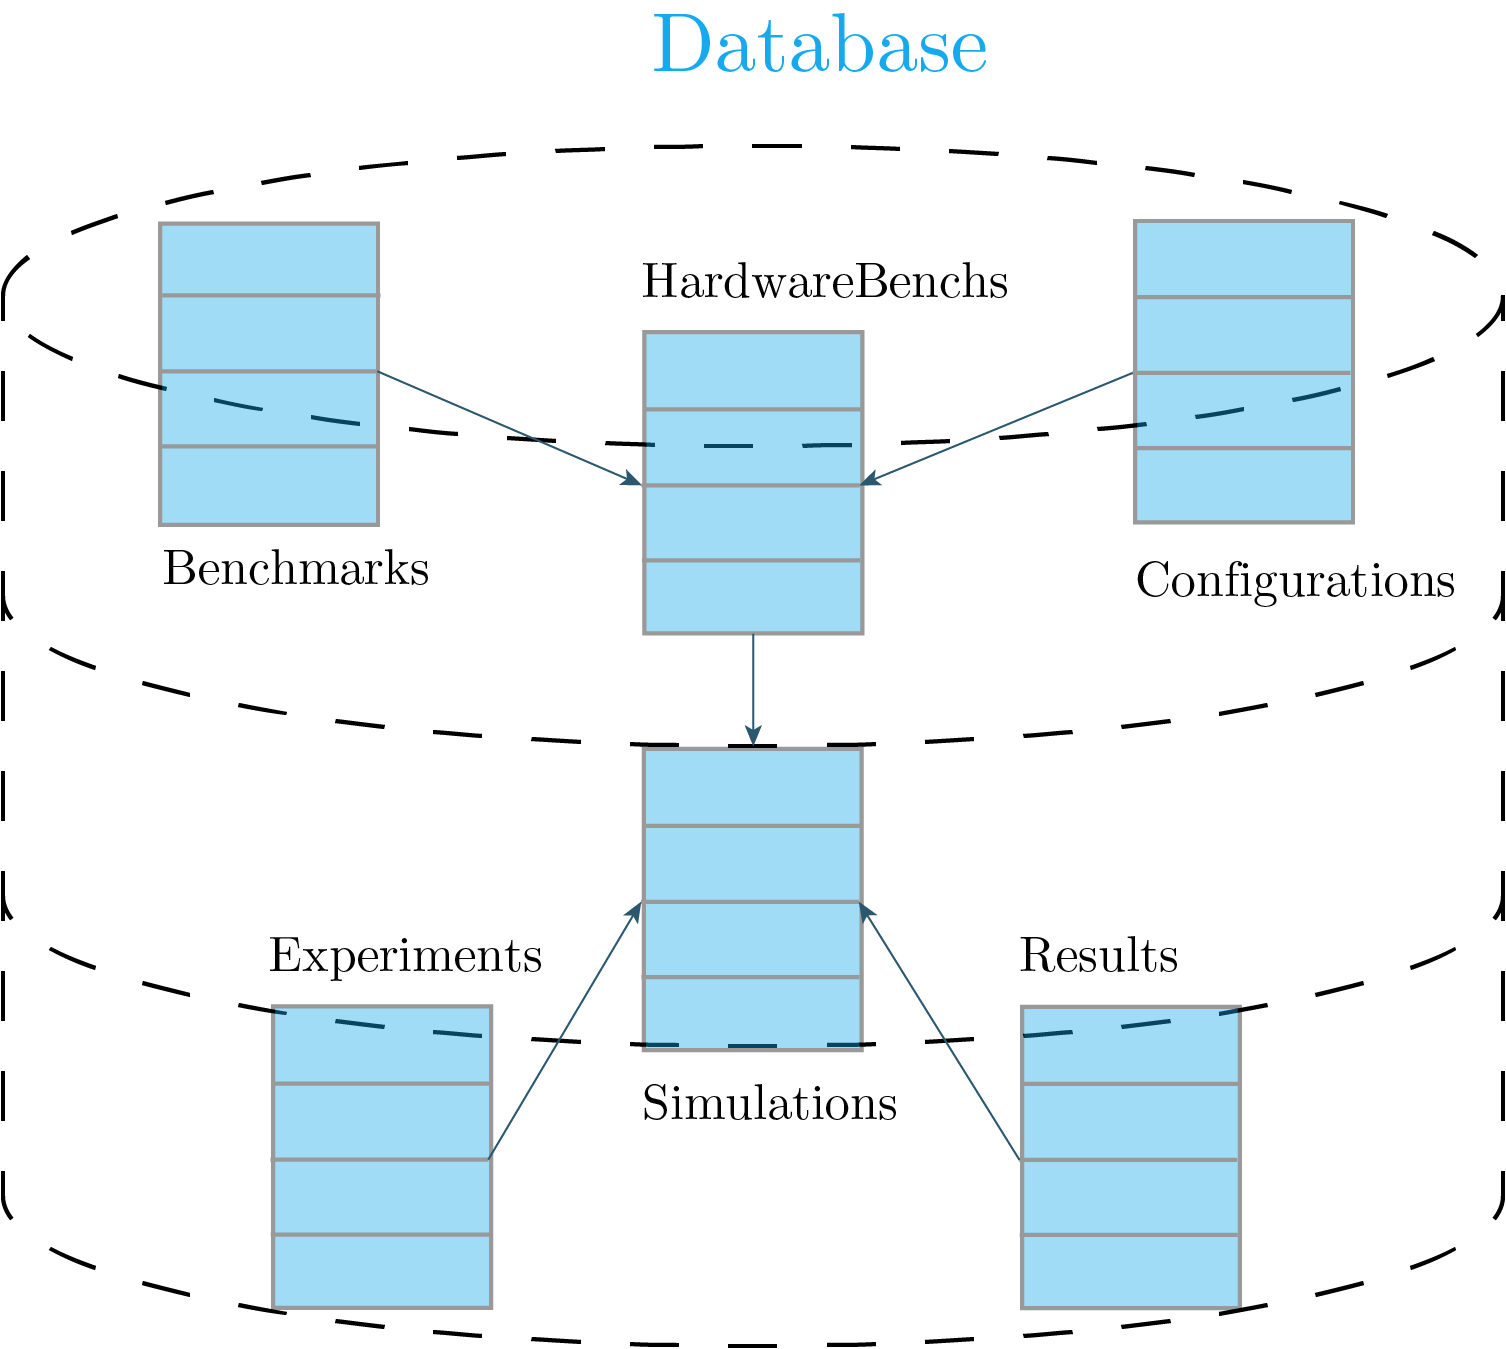
\includegraphics[width=.5\textwidth]{figures/database_scheme_detail.png}
\caption{\label{fig:org8252755}
Database tables}
\end{figure}

\begin{figure}[htbp]
\centering
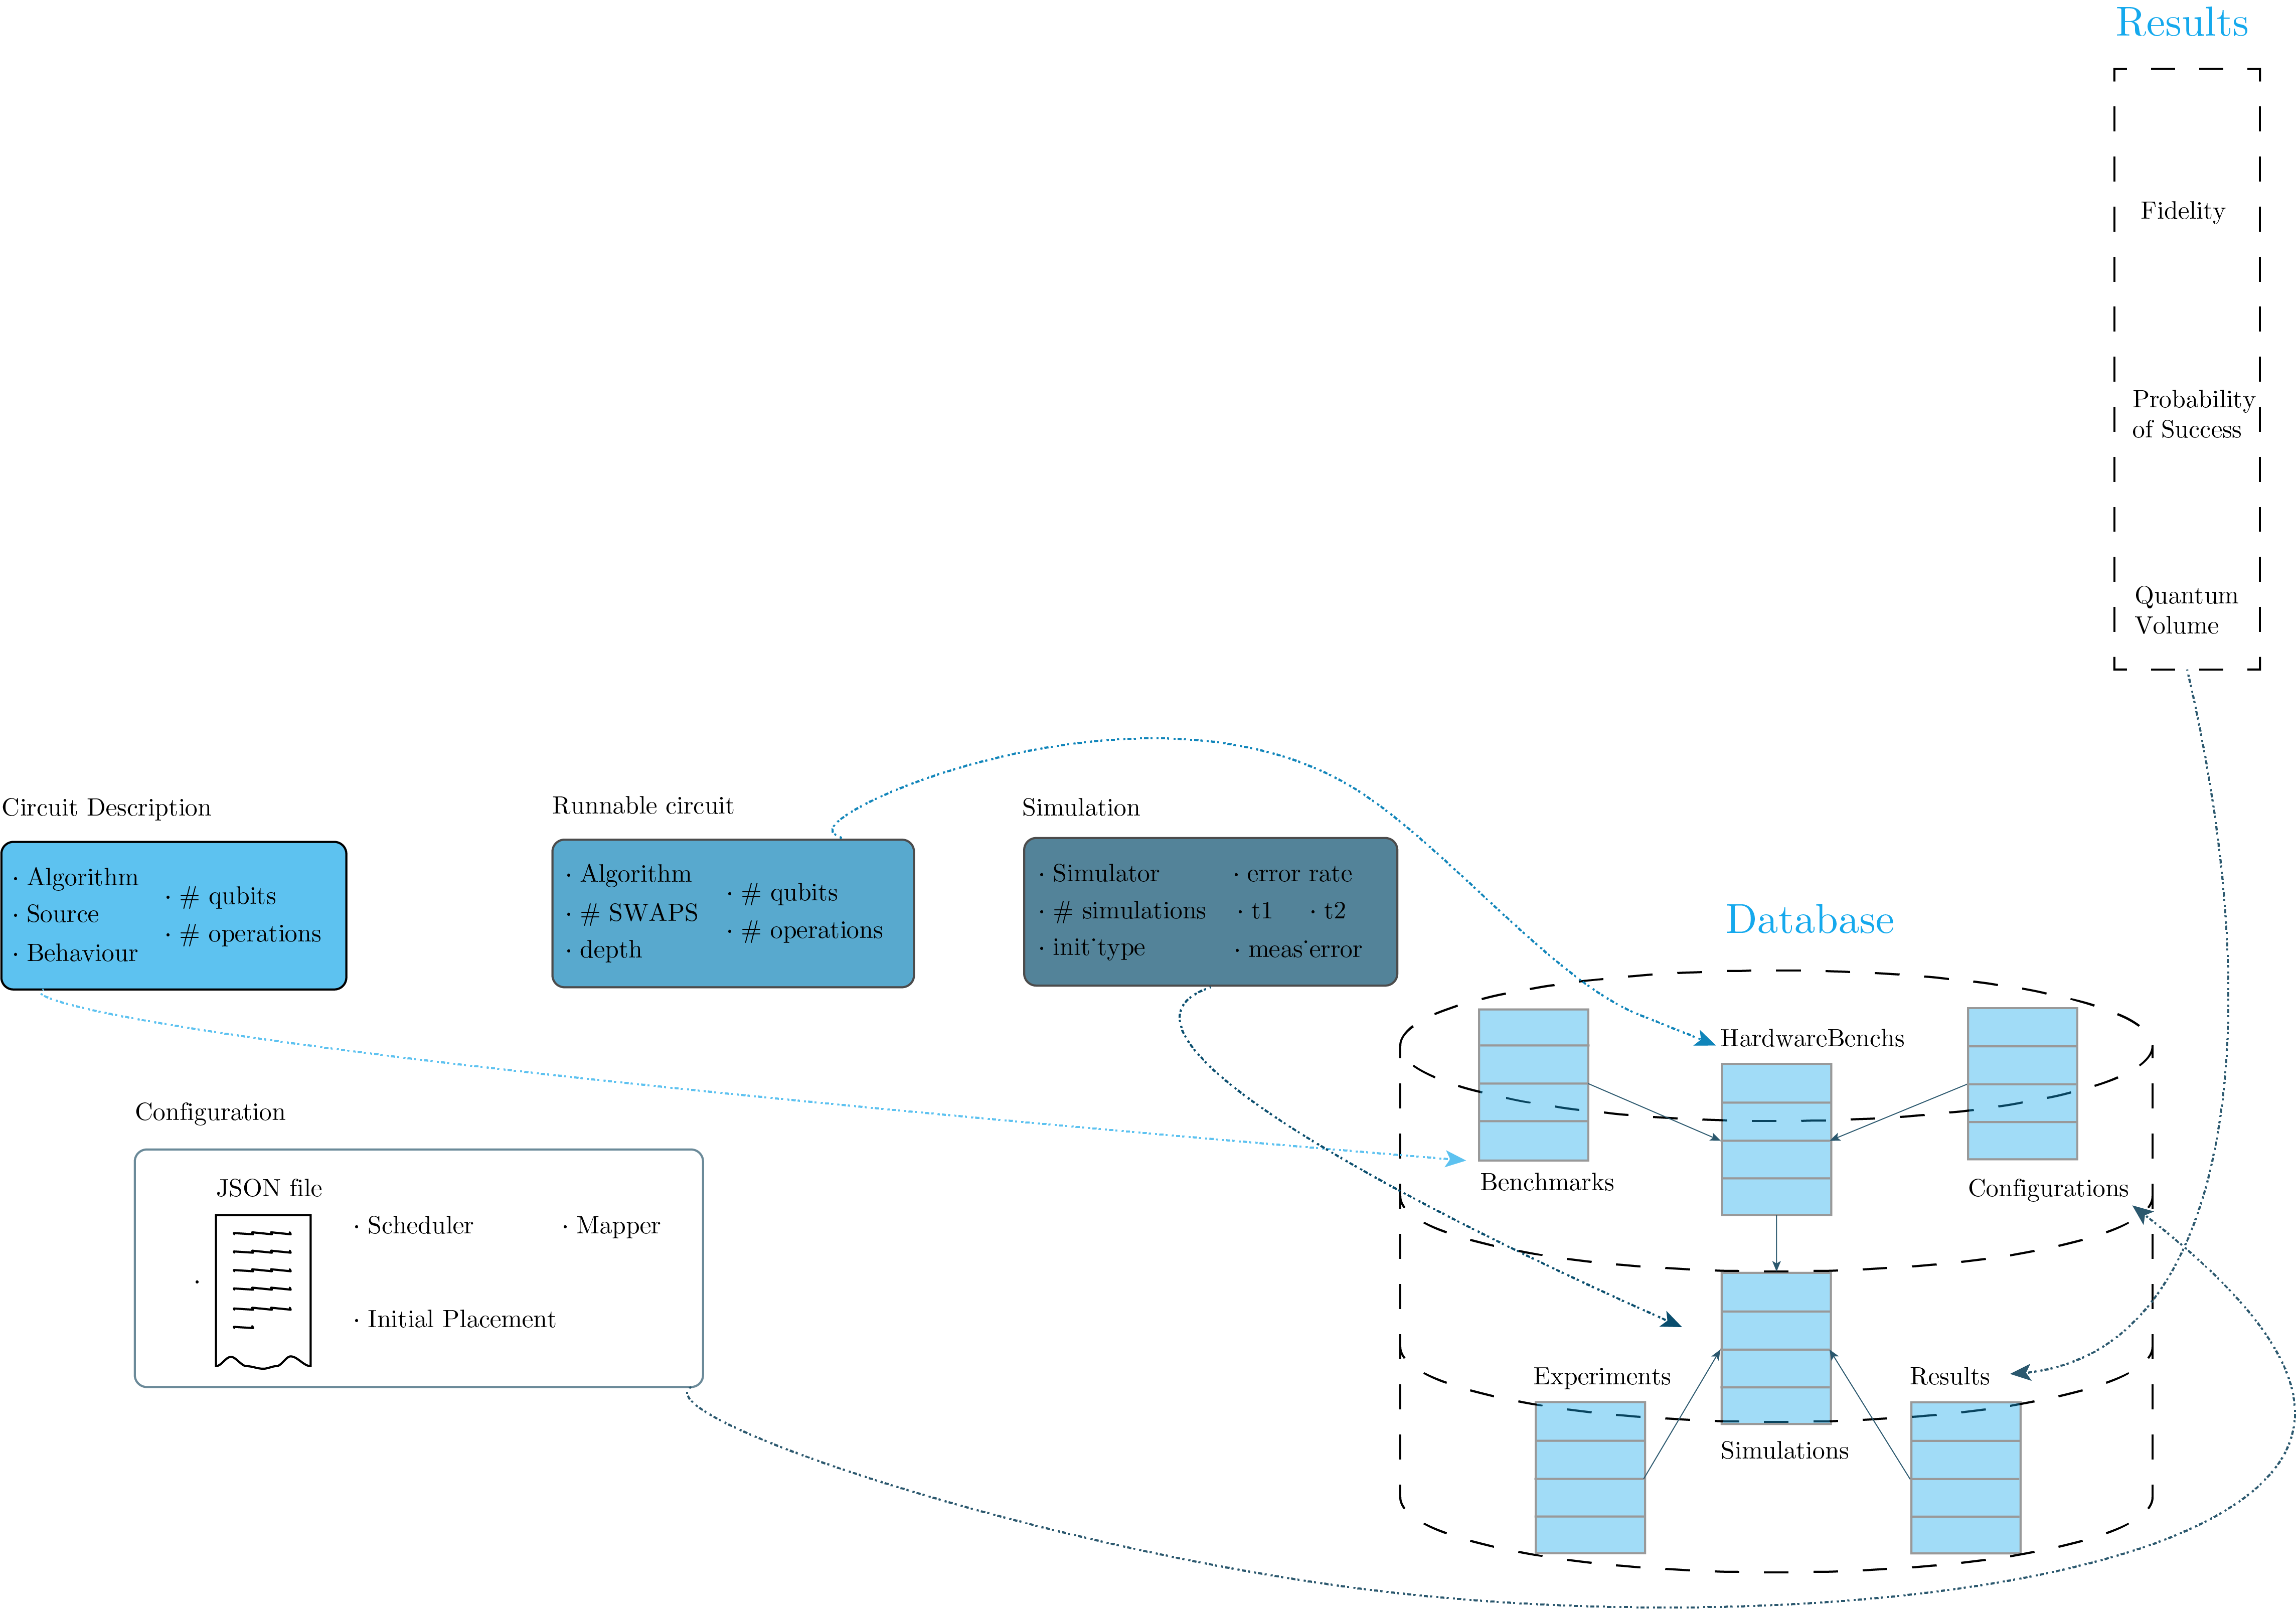
\includegraphics[width=\textwidth]{figures/database_scheme_general.png}
\caption{\label{fig:org8788a51}
Database tables information}
\end{figure}
\end{itemize}
